% ****** Start of file apssamp.tex ******
%
%   This file is part of the APS files in the REVTeX 4.1 distribution.
%   Version 4.1r of REVTeX, August 2010
%
%   Copyright (c) 2009, 2010 The American Physical Society.
%
%   See the REVTeX 4 README file for restrictions and more information.
%
% TeX'ing this file requires that you have AMS-LaTeX 2.0 installed
% as well as the rest of the prerequisites for REVTeX 4.1
%
% See the REVTeX 4 README file
% It also requires running BibTeX. The commands are as follows:
%
%  1)  latex apssamp.tex
%  2)  bibtex apssamp
%  3)  latex apssamp.tex
%  4)  latex apssamp.tex
%
\documentclass[%
 reprint,
%superscriptaddress,
%groupedaddress,
%unsortedaddress,
%runinaddress,
%frontmatterverbose,
%preprint,
%showpacs,preprintnumbers,
%nofootinbib,
%nobibnotes,
%bibnotes,
 amsmath,amssymb,
 aps,
 norsk,
%pra,
%prb,
%rmp,
%prstab,
%prstper,
%floatfix,
]{revtex4-1}

\usepackage[utf8]{inputenc}
\usepackage[norsk]{babel}
\usepackage{varioref}
\usepackage{graphicx}% Include figure files
\usepackage{enumitem}
\usepackage{dcolumn}% Align table columns on decimal point
\usepackage{bm}% bold math
\usepackage[margin=0.9in]{geometry}
\usepackage[mathlines]{lineno}% Enable numbering of text and display math
%\linenumbers\relax % Commence numbering lines

\usepackage[usenames,dvipsnames,svgnames,table]{xcolor}
\usepackage[colorlinks]{hyperref}
\usepackage{relsize}
\usepackage{graphicx,verbatim,amsfonts,geometry}
\usepackage{amsmath}
\newcommand*\diff{\mathop{}\!\mathrm{d}}
\newcommand*\Diff[1]{\mathop{}\!\mathrm{d^#1}}
\usepackage{ulem}
\usepackage{amssymb}
\usepackage{multirow}
\usepackage{soul}
\usepackage{dsfont}
% allows for temporary adjustment of side margins
\usepackage{chngpage}
% just makes the table prettier (see \toprule, \bottomrule, etc. commands below)
\usepackage{booktabs}

\usepackage{commath}
\usepackage{wrapfig}
\usepackage[free-standing-units=true]{siunitx}
\DeclareSIUnit\year{yr}
\usepackage{gensymb}
\newcommand{\ROM}[1]{%
  \textup{\uppercase\expandafter{\romannumeral#1}}%
}
\usepackage{physics}
\usepackage{caption}
\usepackage{bm}
\usepackage{gensymb}
%\usepackage[showframe,%Uncomment any one of the following lines to test
%%scale=0.7, marginratio={1:1, 2:3}, ignoreall,% default settings
%%text={7in,10in},centering,
%%margin=1.5in,
%%total={6.5in,8.75in}, top=1.2in, left=0.9in, includefoot,
%%height=10in,a5paper,hmargin={3cm,0.8in},
%]{geometry}

\begin{document}

%\preprint{APS/123-QED}

\title{Magnetisme}% Force line breaks with \\

\author{Ivar Svalheim Haugerud}

\affiliation{%
 Universitetet i Oslo\\
}%

\date{\today}% It is always \today, today,
             %  but any date may be explicitly specified

\begin{abstract}
Magnetisme er grunnlagget for all elektronikk en bruker i dagens samfunn, og anvendelser av teorien forskes det fortsatt på idag. I denne rapporten studerer vi de magnetiske egenskapene til forskjellige magnetiske materialer, og magnetfelts påvirkning på lys. Vi beregner susceptibiliteten til det diamagnetiske materialet vismut til å være $-1.57\pm0.08$, ved å måle de magnetiske krefter som virker på vistmutstangen.
Videre studerte vi ferromagneten jern, hvor vi måler hvordan geometri og rotasjonsaksen relativt til retningen på magnetfeltet, til jernet, påvirket magnetiseringen av jernet. Jern ble videre studert ved å måle forholdet mellom magnetiseringen og magnetfeltet grunnet strøm i en ytre spole. Målingene viste at jern forsterker styrken på magnetfeltet med rundt en faktor $500$, og at susceptibiliteten til jern ikke er en konstant, men en funksjon av stykren på magnetfeltet. Målinger av Faraday-effekten viste at monokromatiske elektromagnetiske bølger endrer polarisasjonsvinkel av å bevege seg gjennom magnetfelt inne i et flintglass. Fra målingene kunne vi beregne Verdet-konstanten for tre forskjellige bølgelengder, $440, 580, \SI{595}{\nano\meter}$, som ga oss en verdi på henholdsvis $\SI{135\pm2}{\deca\degree/\tesla\meter}$, $\SI{140\pm1}{\deca\degree/\tesla\meter}$, og $\SI{119\pm1}{\deca\degree/\tesla\meter}$.
For bølgelengdene på $580, \SI{595}{\nano\meter}$ stemte målingene med teorien, men ikke for lys med bølgelengde $\SI{440}{\nano\meter}$ grunnet systematiske feil, det burde derfor gjennomføres fler eksperimenter for Verdet-konstanten for bølgelengder rundt denne.
\end{abstract}

\pacs{Valid PACS appear here}% PACS, the Physics and Astronomy
                             % Classification Scheme.
%\keywords{Suggested keywords}%Use showkeys class option if keyword
                              %display desired
\maketitle

%\tableofcontents

\section{Introduksjon}
Magnetisme er et fenomen mennesker har vist om, og utnyttet i lang tid. Thales fra Milet kjente til de magnetiske egenskapene til magnetjernstein, mer enn $500$ år før kristus \cite{holtebekk_magnetisme_2017}. En anvendelse av magnet ble ikke funnet før på $800$-tallet, hvor mennesker navigerte med kompass for første gang \cite{holtebekk_magnetisme_2017}. Det tok $1000$ år til før det kom en beskrivelse av magneter ved Faraday og Maxwell, som virkelig tok anvendelsen til en ny skala. Fysikeres forståelse av magnetisme har gjort mulig den teknologiske revolusjonen som påvirker dagliglivet vårt. Datamaskinen jeg skriver dette på ville ikke fungert uten anvendelsen av magnetisme på en liten skala. Elektriske motorer, generatorer, medisinsk teknologi og mobiltelefoner er bare noen få eksempler på anvendelser av magnetisme. Selv om magnetisme er en anvendelig teori, er det også en fundamental teori. Det er bevegelsen av ladde partikler som danner magnetiske felt, og ladde partikler er en del av de fleste fysiske teorier. Forståelsen vår av magneter er ikke fullført, og det forskes fortsatt på magnetiske egenskaper i materialer, superledere, som har svært spesielle magnetiske egenskaper, innen medisinsk forskning, og mye mer.
I denne rapporten er det fokus på magnetismens effekt, i og av, materialer. Og dette skal vi studere ved å gjennomføre eksperimentelle målinger, og teste målingene opp mot teori innenfor elektromagnetisme.\par
Eksperimentet i denne rapporten ble gjennomført i håp om å forstå forskjellige egenskaper til diamagneter og ferromagneter, og måle magnetismens innvirkning på lys. For å gjøre dette ble det gjennomført eksperimentelle målinger, som består av tre forskjellige hoveddeler.\\
Først ønsker vi å beregne den magnetiske susceptibiliteteten til en vismutstang ved å bruke et eksternt magnetfelt, og måle den magnetiske kraften som virker på vistmutstangen. Deretter skal vi studere ferromagnetiske materialer ved å måle magnetiseringen av jern med to forskjellige utgangspunkter. Tilslutt skal vi studere Faraday-effekten, hvordan polarisert, monokromatisk, lys endrer polarisasjonsvinkel av å bevege seg gjennom et ytre magnetfelt i et materiale. Disse eksperimentene skal gi oss en innsikt i magnetiske materialer, og deres innvirkning på lys.
\section{Teori}
Hele den klassiske elektromagnetismen kan beskrives ved hjelp av fire partsielle differensiallikninger. Disse likningene beskriver elektriske $\bm{E}$ og magnetiske $\bm{B}$ felt, og forklarer Lorentz kraften, klassisk optikk og elektriske kretser. Likningene kan skrives på flere måter, og på flere former. I denne rapporten velger vi å bruke følgende:
\begin{align}
  \nabla \cdot \bm{E} &= \frac{\rho}{\epsilon_0} \label{1}\\
  \nabla \cdot \bm{B} &= 0 \label{2}\\
  \nabla \cross \bm{E} &= -\pdv{\bm{B}}{t} \label{3}\\
  \nabla \cross \bm{B} &= \mu_0\left(\bm{J} + \epsilon_0\pdv{\bm{E}}{t}\right) \label{4}
\end{align}
I likningene er $\rho$ den elektriske tettheten, og $\epsilon$ er permittiviteten, som beskriver motstanden et medie har mot et påtrykt elektrisk felt. I disse likningene brukes $\epsilon_0$, som er en naturkonstant, som angir permittiviteten i vakum. $\mu$ er et mål på matrialers evne til å magnetiseres av et ytre påtrykket magnetfelt. I disse likningene brukes vakuumpermeabiliteten $\mu_0$ som er en naturkonstant, som angir permeabiliteten i vakum. Permeabiliteten i et materiale kan skrives som produktet av vakuumpermeabiliteten, og den relative permeabiliteten $\mu_r$. Fra dette kan en få den dimensjonsløse verdien magnetiske susceptibilitet $\chi = \mu_r - 1$. Den magnetiske susceptibiliteten forteller oss hvordan materialet blir magnetisert av et ytre påtrykt magnetisk felt, og brukes til å klassifisere hva slags magnetisk materiale vi ser på. $\bm{J}$ beskriver strømtetthet, det vil si elektrisk strøm $I$ gjennom et flateareal $A$. \\
Maxwell's likninger kan også skrives ved $\bm{H}$-feltet istedenfor $\bm{B}$-feltet. Hvor $\bm{B}$-feltet representerer den totale magnetiske flukstettheten, fra alle kilder, men $\bm{H}$-feltet bare magnetfelt fra frie strømmer, og derfor ikke fra magnetisering til materialer $\bm{M}$. Definisjonen av $\bm{H}$-feltet blir da
\begin{equation}
  \bm{H} = \frac{\bm{B}}{\mu_0}-\bm{M}, \label{get_H}
\end{equation}
Maxwell's likninger kobler sammen elektriske og magnetiske felt. Magnetiske felt stammer fra elektrisk ladde partikler i bevegelse. I atomer beveger elektroner seg i bane rundt atomet, og danner et magnetfelt fra angulærmomentet. Elektronet har også en egenspinn, som gjør at elektronet kan sees på som et dipol. Hvordan angulærmomentet til de forskjellige elekronene rundt materialet er satt sammen, avgjør de magnetiske egenskapene til materialet atomet består av. Dette resulterer i forskjellige typer magnetiske materialer: diamagnetiske, paramagnetiske og ferromagnetiske.
\subsection{Diamagnetisme}
De aller fleste materialer er ikke magnetiske. Slike materialer kaller vi for diamagnetiske materialer, som klassifiseres ved at de ikke er magnetiske, uten en ytre påvirkning. Diamagnetiske materialer kan bli magnetisert ved å påtrykke et ytre magnetfelt, som deformerer elektronorbitalene. Ved Lenz regel vil dette generere et magnetfelt som motsetter seg forandringen av feltstyrken. Dette betyr at diamagnetiske materialer danner et magnetfelt som motsetter seg det ytre påtrykte magnetfeltet, derfor er susceptibiliteten til diamagnetiske materialer negativ, $\chi < 0$. Lenz regel gjelder for alle atomer, og følgelig alle materialer, men denne effekten er svært liten i forhold til andre magnetiske effekter. Selv om dette er en liten effekt er den viktig, siden dette gjelder alle materialer.\\Det kan vises, med utgangspunkt i potensiell energi for en magnetisk dipol, med dipolmoment $\mu$, i et magnetfelt, at den magnetiske kraften som virker er gitt av
\begin{equation}
  F_Z = -\frac{\chi}{2\mu_0}A\left(B_1^2 - B_2^2\right). \label{vismut}
\end{equation}
Hvor $B_1$ og $B_2$ er magnetfeltet på tvers av symmetriaksen til stangen, i henholdsvis bunn og toppen av stangen, og $A$ er tverrsnittsarealet. Dette kan løses for susceptibiliteteten, og skrives som
\begin{equation}
  \chi = \frac{2\mu_0F_z}{B_1^2 - B_2^2}.
\end{equation}
Under eksperimentet er det to forandringer ved denne funksjonen vi ønsker å teste konsekvensene av. Vi ønsker å studere hvordan susceptibiliteteten endrer seg ved å anta et lineært forhold mellom kraften $F_z$ og susceptibiliteteten, slik at susceptibiliteteten kan skrives som
\begin{equation}
  \chi = \frac{2\mu_0F_z}{B_1 - B_2}.\label{lin_chi}
\end{equation}
Vi ønsker også å se om tilnærmingen $B_2=\SI{0}{\tesla}$ er en god tilnærming under beregningen av $\chi$. Det kan vises at endringen i susceptibiliteteten $\Delta \chi$ ved å anta $B_2=\SI{0}{\tesla}$ er gitt av
\begin{equation}
  \frac{\Delta \chi}{\chi} = \frac{B_2^2}{B_1^2}. \label{test_chi}
\end{equation}
Dette uttrykket kan vi bruke for å teste om tilnærmingen $B_2=0$ er god eller ikke.
\subsection{Paramagnetisme og ferromagnetisme}
I diamagnetiske materialer kansellerte spinnet til elektronene slik at netto angulært moment er tilnærmet null. For andre materialer, hvor spinnet til elektronene ikke kansellerer hverandre, vil bevegelsen til elektronene danne et netto magnetisk moment. Er den gjennomsnittlige orienteringen til atomenes magnetfelt i en bestemt retning, vil summen av alle magnetfeltene danne et magnetisk felt som kan merkes utenfor mediet. Dette betyr at materialet er \textit{magnetisert}, som beskrives med paramteren $\bm{M}$. Materialer som oppfører seg slik klassifiseres som paramagnetiske og ferromagnetiske materialer.\par
Paramagnetiske materialer vil ikke kunne danne et magnetfelt alene, og klarer det kun fra et ytre påtrykt magnetisk felt. Det ytre påtrykte magnetfelt vil få alle de magnetiske dipolene i materialet til å rette seg i samme retning. Fjernes feltet vil orienteringen bli tilfeldig igjen, og materialet vil ikke lenger danne et magnetisk felt. Magnetiseringen av materialet er omtrent proposjonalt med styrken på det ytre påtrykte magnetfeltet $\bm{H}$, $\bm{M} = \chi\bm{H}$, hvor den magnetiske susceptibiliteten $0<\chi\ll1$. En paramagnet forsterker det påtrykte magnetfeltet.
\par
Ferromagnetiske materialer oppfører seg som paramagnetiske materialer, men størrelsen på magnetiseringen er mye større. Forsterkningen av det ytre påtrykte magnetfeltet kan være opp mot en faktor $10 000$ sterkere \cite{oppgave}. Den sterke magnetiseringen fører til at de atomære dipolene klarer å opprettholde magnetfeltet sitt, etter at det ytre magnetfeltet er fjernet. Dette betyr at man kan lage en permanentmagnet ved å magnetisere et ferromagnetisk materiale. For ferromagneter er den magnetiske susceptibiliteten ikke en materialkonstant. Det er ikke et lineært forhold mellom det ytre påtrykte magnetfeltet og den magnetiske susceptibiliteten, susceptibiliteten er avhengig av geometrien og retningen til materialet, og styrken på det påtrykte magnetfeltet.
\par
For å avmagnetisere et ferromagnetisk materiale trengs det et magnetisk felt, styrken på mangetfeltet som trengs kalles avmagnetiseringsfeltet $\bm{H}_d$, er gitt av
\begin{equation}
  H_{i, d} = D_iM_i,
\end{equation}
for ellipsoider med uniform magnetisering. I likningen representerer indeksen $i$ en retning $(x, y, z)$, og $D_i$ er avmagnetiseringsfaktoren. Avmagnetiseringsfaktoren kan beregnes analytisk fra å vite formen på ellipsoiden. Formen på ellipsoiden kan klassifiseres ved ett tall, eksentrisiteten $\epsilon$, som er gitt av
\begin{equation}
  \epsilon = \sqrt{1-\frac{1}{f^2}},\label{eksent}
\end{equation}
hvor $f$ er gitt av
\begin{equation}
  f = \frac{a_{\parallel}}{a_{\perp}}.
\end{equation}
I likningene er $a_{\parallel}$ lengden parallelt med rotasjonsaksen til ellipsoiden, og $a_{\perp}$ er lengden til ellipsoiden ortogonalt på rotasjonsaksen. Fra å vite eksentrisiteten til ellipsoiden kan en beregne avmagnetiseringsfaktoren parallelt med $D_{\parallel}$, og ortogonalt på $D_{\perp}$, rotasjonsaksen
\begin{align}
  D_{\parallel} &= \left(1-\frac{1}{\epsilon^2}\right)\left(1-\frac{1}{2\epsilon}\ln{\left(\frac{1+\epsilon}{1-\epsilon}\right)} \right) \\
  D_{\perp} &= \frac{1-D_{\parallel}}{2}
\end{align}.
\par
Det er ikke mulig å måle $\bm{H}$, eller $\bm{M}$-feltet, det eneste vi kan måle er magnetisk flukstetthet $\bm{B}$. Og vi kan ikke finne et analytisk uttrykk for hvordan den magnetiske flukstettheten $B$ varierer med den opprinnelige flukstettheten $B_0$, kan vi finne en øvre og nedre grense for styrken på den magnetiske flukstettheten
\begin{equation}
  B_0 < B_i < \frac{B_i}{D_i}, \label{upper_limit}
\end{equation}
hvor indeksen $i$ viser til symmetriaksen til jernklumpen er parallell med eller ortogonalt på retningen til magnetfiltet.
\\Under eksperimentet kommer magneten til å bli plassert i en spole med $N$ vinninger, og lengde $L$, med en strøm $I$ som går gjennom. Da vil den magnetiske flukstettheten i sentrum av spolen være gitt av
\begin{equation}
  B = \frac{\mu_0NI}{L}. \label{nice_b}
\end{equation}Den teoretiske verdien kan vi teste mot målingene vi gjør av den magnetiske flukstettheten under eksperimentet. Dette betyr at styrken på $H$-feltet generert av samme spole er gitt av
\begin{equation}
  H = \frac{NI}{L}. \label{nice_H}
\end{equation}
\par
I eksperimentet kommer vi til å måle den magnetiske flukstettheten på en mer direkte måte ved å studere magnetiseringen av jern. For å gjøre dette kommer vi til å bruke en spenningsgenerator som gir oss integralet av forskjellen i elektrisk potensial $\epsilon$, mellom endepunktene til en sekundærspole, som ligger inne i en primærspole,
\begin{equation*}
  \Delta S = \frac{1}{\kappa}\int_{t_0}^{t}\epsilon \diff \tau, \label{deltas}
\end{equation*}
hvor $\kappa$ er en kalibreringskonstant. Spenningen over strømsløyfen vil generere et tidsvarierende magnetfelt fra Faraday's induksjonslov \eqref{3}. Fra å integrere Faraday's induksjonslov \eqref{3} finner man en lineær sammenheng mellom endringen av magnetisk fluks $\Delta \Phi$ og utslaget til spenningsgeneratoren $\Delta S$. Fra å vite tverrsnittsarealet $A$, og antall vindinger $n$ til sekundærspolen, kan en da beregne endringen i magnetisk flukstetthet
\begin{equation}
  \Delta B = \frac{\kappa\Delta S}{nA}.\label{deltab}
\end{equation}
\subsection{Faraday-effekten}
Faradayeffekten er et magneto-optisk fenomen hvor et plan av polarisert lys blir polarisert av å bevege seg gjennom et medium som er i et magnetisk felt. Mengden lyset blir polarisert er et produkt av lengden til mediet det reiser gjennom, $L$, styrken på magnetfeltet i mediet, $B$, og en proposjonalitetskonstant som kalles \textit{Verdet-konstanten}, $V$. Med dette blir uttrykket for polarisasjonsvinkelen
\begin{equation}
  \theta\left(B, L, \lambda\right) = V\left(\lambda\right)LB.\label{verdet}
\end{equation}
Verdet-\textit{konstanten} er uavhengig av lengden til krystallen og magnetfeltet, men er avhenig av bølgelengden, $\lambda$, til lyset, og er følgelig bare en konstant for bestemte bølgelengder.\\
%Årsaken til Faraday-effekten har sine røtter i den kvantemekaniske verden, men kan forklares, på et grunnleggende nivå, ved hjelp av klassisk elektrodynamikk. Elektrodynamikken spår at Verdet-konstanten er en funksjon av bølgelengden til lyset \cite{pdf_task}
%\begin{equation}
%  V = \frac{2be}{m_ec\lambda^2}, \label{test_verdu2}
%\end{equation}
%hvor $e$ er elementærladningen, $m_e$ massen til et elektron, og $c$ lyshastigheten i vakum, og $b$ er en konstant lik $\SI{8920}{\naon\meter^2}$. Denne funksjonen gir deg Verdetkonstanten i radianer per tesla meter. Dette uttrykket ønsker vi å sammenlikne med den eksperimentelle verdien for Verdet-konstanten.
\subsection{Usikkerhet}
Når vi regner med størrelser med usikkerhet, må usikkerheten følge videre fram til svaret. For å gjøre dette bruker vi regneregler for usikkerheter \cite{squires}. Hvor usikkerheten i $Z=A+B$ er gitt av
\begin{equation*}
  \Delta Z = \sqrt{\Delta A^2+\Delta B^2},
\end{equation*}
hvor usikkerheten til størrelsene blir vist som $\Delta$ foran størrelsen. For produktet mellom to størrelser $Z=A\cdot B$, blir usikkerheten gitt av
\begin{equation*}
  \Delta Z = Z\sqrt{\left(\frac{\Delta A}{A}\right)^2 + \left(\frac{\Delta B}{B}\right)^2}.
\end{equation*}
Når det kommer til logaritmer $Z=\log{A}$, er usikkerhet gitt av
\begin{equation*}
  \Delta Z = \frac{\Delta A}{A}.
\end{equation*}
Disse tre regnereglene kombinerer vi gjennom hele oppgaven for beregning av usikkerhetene. Usikkerheten i en enkelt måling finner vi fra databladet til måleapparatet brukt under målingen. Under beregning av stigningstall, med usikkerhet, bruker vi fremgangsmåten gitt av G. L. Squires \cite{squires}. For flere målinger av samme verdi tar vi hensyn til målingen av hver enkelt måling, og spredningen til målesettet.
\par
Under eksperimentet kommer vi til å teste om flere av de målte verdiene våre stemmer overens med teoretiske prediksjoner. Vi forventer ikke at differansen mellom den teoretiske og eksperimentelle verdien er null, grunnet måleusikkerheter. Men vi ønsker at differansen $D$ skal være mindre enn usikkerheten i differansen $\Delta_D$. For at vi skal ha \textit{overenstemmelse innenfor måleusikkerhetene} må differansen til den eksperimentelt målte verdien, og den forventet teoretisk verdien, tilfredstille
\begin{equation}
  D < \Delta D, \label{usikk1}
\end{equation}
der
\begin{equation}
  \Delta_D = \sqrt{\Delta E_1^2 + \Delta E_2^2}. \label{usikk2}
\end{equation}
Hvor $\Delta E_1$ og $\Delta E_2$ er usikkerheten til den eksperimentelle og teoretiske verdien.
Hvis målingene våre tilfredsstiller denne ulikheten kommer årsaken til differansen $D$ mest sannsynlig fra usikkerheter i målemetoden og tilfeldige feil.
\section{\label{sec:level3}Eksperimentelt}
\subsubsection{Utstyrsliste}
\begin{itemize}
  \item Multimeter (Fluke 45)
  \item Hallsonde (TEL-Atomic Smart magnetic sensor model SMS 102, og Frederiksen 4060.50 teslameter)
  \item Presisjonsvekt (Highland HCB602H)
  \item Strømkilde (Delta Elektronika Power Supply 3004-D)
  \item Spenningsgeneratoren (TTi TG1006 DDS FUNCTION GENERATOR)
  \item Dataakvisasjonsboks (Paspoint Voltage Current sensor - usb link)
  \item Flintglass (PHYWE SF6 cylinder)
  \item Fargefilter (PHYWE 440, 580, 595nm)
  \item Skyvelær
  \item To Polarisasjonsfiltere
  \item Elektrisk spole
  \item Jernklumper, i fire forskjellige former
  \item Jernsylinder
\end{itemize}
\subsection{Diamagnetisme}
I dette eksperimentet ønsker vi å bestemme den magnetiske susceptibiliteten $\chi$ til en vismutstang. Dette gjøres ved å plassere en vismutstang, som er det mest diamagnetiske metallet vi kjenner, i et homogent magnetfelt, og måle kraften som virker på vismutstangen. En illustrasjon av det eksperimentelle oppsettet er vist i figur \vref{eksperimentelt_oppsett1}. For å genere et magnetfelt ble det brukt to elektriske spoler på hver side av vismutstangen, som en ser i figur \vref{eksperimentelt_oppsett1}. På denne måten kunne vi variere strømmen i kretsen for å variere styrken på magnetfeltet. Vismutstangen ble plassert i magnetfeltet slik at bunnen av stangen var i sentrum av de to spolene, slik en kan se i figuren.
\begin{figure}[h!]
  \centering
  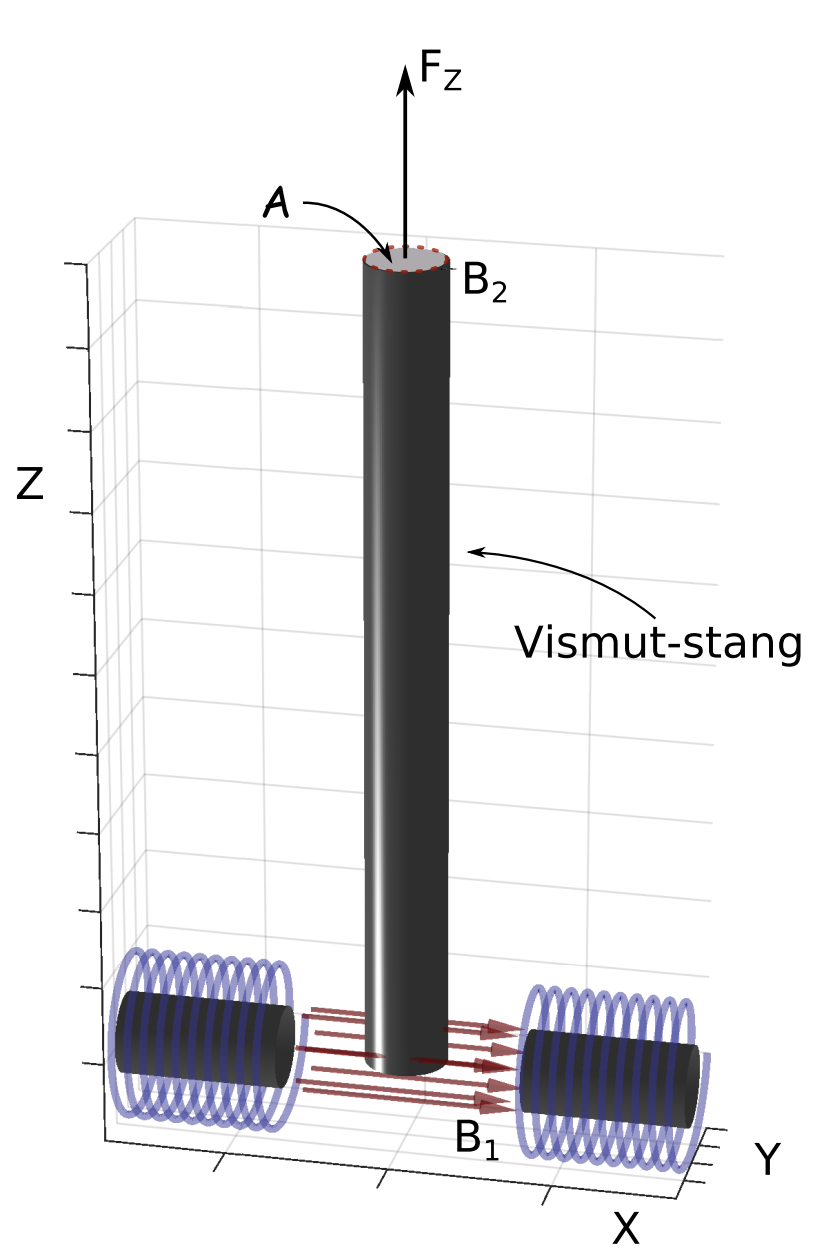
\includegraphics[scale=0.38]{oppsett1.png}
  \caption{Illustrasjon av vismutstang i magnetfelt brukt for å måle magnetisk susceptibilitet i vismut. I figuren ser vi de forskjellige størrelsene som blir målt under eksperimentet, styrken på magnetfeltet mellom spolene $B_1$, styrken på magnetfetlet ved enden av vismutstaven $B_2$, tverrsnittsarealet til vismuststaven $A$ og den magnetiske kraften som virker på vismutstangen $F_z$, for å kunne beregne susceptibiliteten. De blå sirklene representerer strømspolen som generer magnetfeltet. Fiugren er hentet fra fysisk institutt, universitetet i Oslo \cite{oppgave}.}
  \label{eksperimentelt_oppsett1}
\end{figure}
Under eksperimentet varierte vi strømmen i kretsen fra $\SI{0}{\ampere}$ til $\SI{2.4}{\ampere}$, med en lineær økning på $\SI{0.2}{\ampere}$. Den magnetiske kraften som virker på vismut staven er gitt av \eqref{vismut}, som gjør at vi trenger å måle tverrsnittsarealet $A$, den magnetiske kraften $F_z$, og magnetfeltet $B_1$ og $B_2$ for å kunne beregne susceptibiliteten. Tverrsnittsarealet beregnes ved å måle diameteren til stangen med et skyvelær. Målingen av diameteren ble gjort på flere punkter langs vismutstangen, itilfelle tverrsnittsarealet ikke var konstant over stangen. Magnetfeltet måles uten at vismut staven er i magnetfeltet, ved å feste en Hallsonde, og lese av målingen til Hallsonden mens vi varierer strømstyrken. Dette måtte gjøres to ganger, med hall-soden på to forskjellige posisjoner, for å måle magnetfeltet mellom spolene $B_1$, og magnetfeltet på enden av vismutstaven $B_2$. \\
Vistmutstangen er festet i et tau, dette tauet festes i en krok. Denne kroken hviler på en presisjonsvekt. Før det går strøm i spolen nullstiller vi vekten, og lese av endringen i vekt som funksjon av strømstyrke, som gjør at vi kan beregne $F_z$ som en funksjon av strømstyrken. Dette gir oss muligheten til å finne en verdi for susceptibiliteteten til vismut.
\subsection{Ferromagnetisme}
I denne delen av eksperimentet ønsker vi å undersøke magnetisering av ferromagneten jern på to forskjellige måter. Først ønsker vi å studere jernklumper inn i en spole, og måle påvirkningen geometri og retning har på magnetfeltet, og deretter studere magnetiseringen av en jernsylinder med en varierende strømforskyvning, ved hjelp av Faradays induksjonslov. \par
Først skal vi gjøre målinger på fire forskjellige jernklumper med ulik geometri inne i en stor spole, som generer et tilnærmet homogent magnetfelt på innsiden. Spolen har $244$ vindinger, og en lengde på $\SI{275}{\milli\meter}$. Jernklumpene har fire forskjellige geometrier vi ønsker å studere: kule, stang, spiss, avlang ellipsoide, og skive. En illustrasjon av oppsettet brukt under eksperimentet er vist i figur \vref{eksperimentelt_oppsett2}.
\begin{figure}[h!]
  \centering
  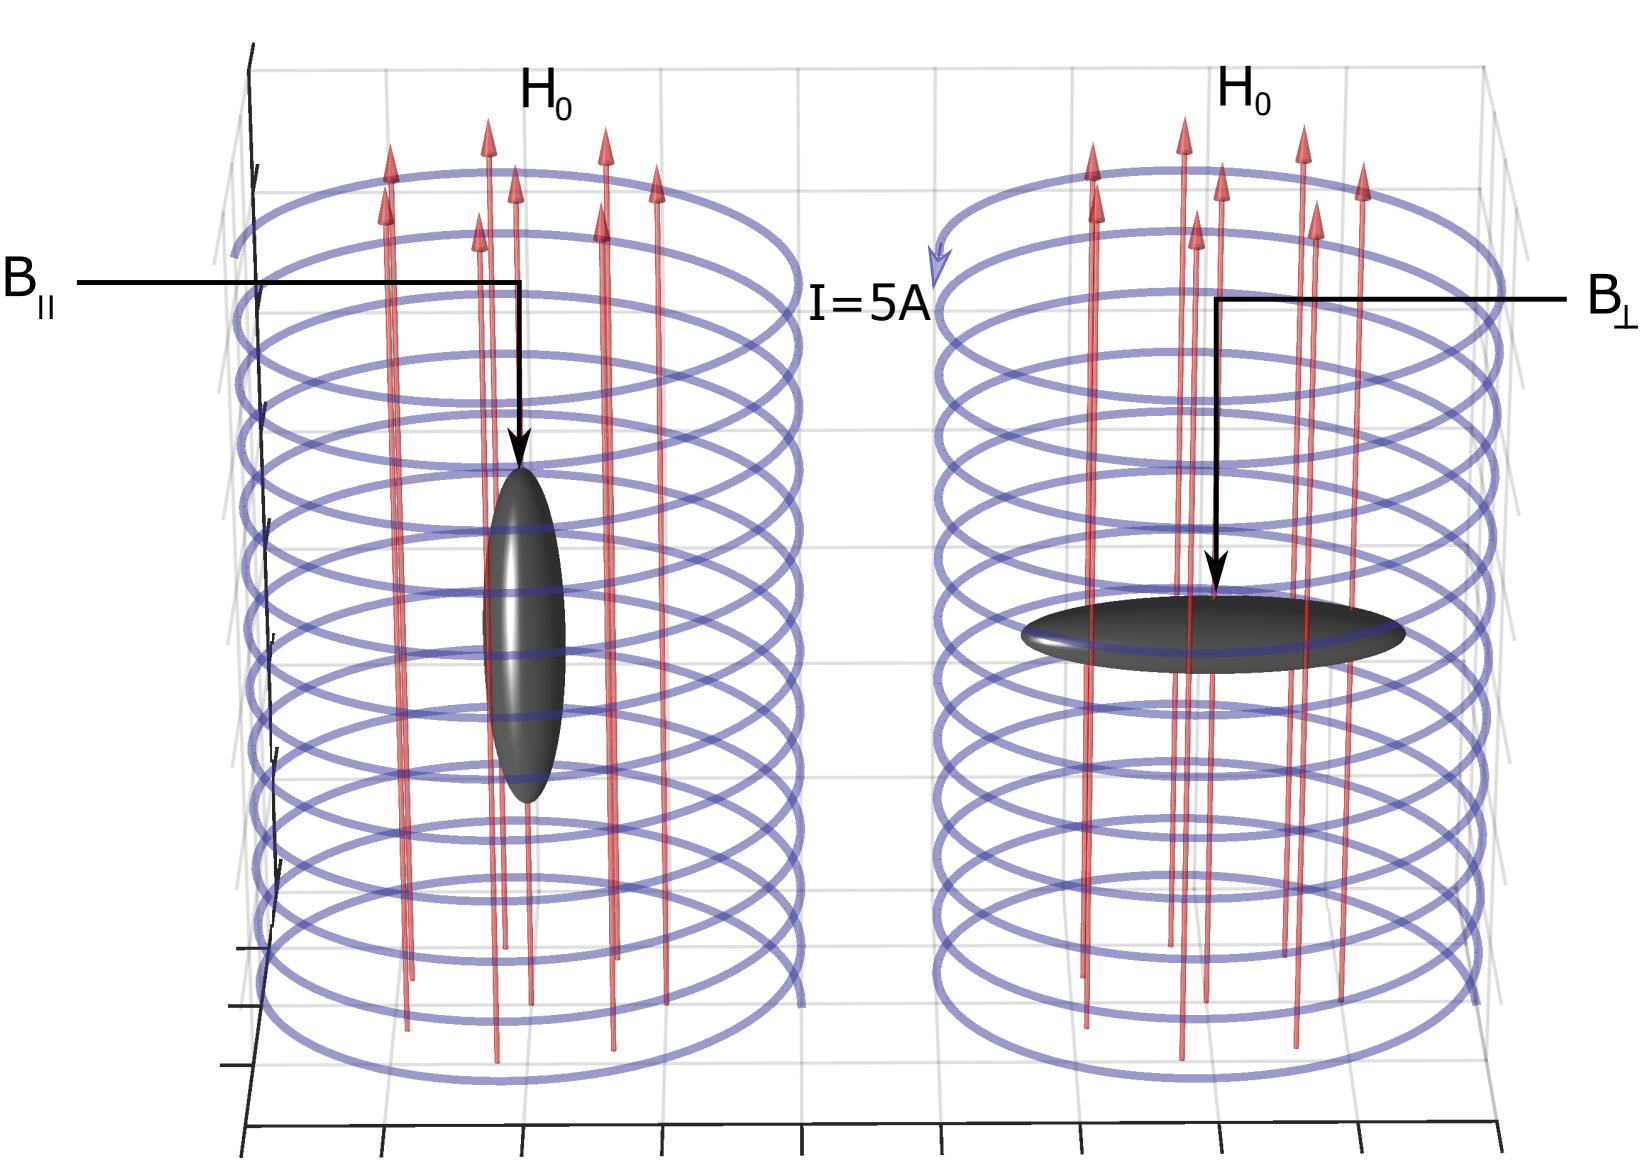
\includegraphics[scale=0.24]{oppsett2.png}
  \caption{Illustrasjon av jern ellipsoiden inne i en spole. I figuren er det vist med rotasjonsaksen til jernklumpen parallelt med magnetfelt (venstre), og rotasjonsaksen til jernklumpen ortogonalt på magnetfeltet (høyre). De røde linjene viser retningen på magnetfeltet, og de blå linjene viser spolen som jernklumpen blir plassert i. Fiugren er hentet fra fysisk institutt, universitet i Oslo \cite{oppgave}.}
  \label{eksperimentelt_oppsett2}
\end{figure}
Før vi gjør målinger med jernklumpene inne i spolen, måler vi magnetfeltet inne i spolen, når det går en strøm på $\SI{5}{\ampere}$, forskjellige steder i spolen. Dette blir gjort ved hjelp av en Hallsonde. Under målingene passer vi på at hallsonden står normalt på magnetfeltet, for å få mest presise målinger.\\For å ha jernklumpene i sentrum av spolen blir det brukt plastikkstativ som plasseres inne i spolen. Vi gjentar derfor målingene av magnetfeltet med Hallsonden, men nå med plastikkstativet for å teste om dette påvirker magnetfeltet inne i spolen. For å vite eksentrisiteten til de fire geometriske formene gjorde vi målinger av lengden til objektene langs, og på tvers av, rotasjonsaksene, med skyvelær. Fra disse verdiene kunne vi beregne eksentrisiteten ved \eqref{eksent}.\\
Deretter ble det gjennomført målinger av magnetfeltet på overflaten til hver av de fire jernklumpene, mens de var plassert i spolen, med strømmen til spolen på. På grunn av Gauss lov for magnetfelt måler vi styrken på innsiden av materialet ved å måle rett på utsiden. Målingene ble gjort for hver av klumpene med rotasjonsaksen parallelt med magnetfeltet, og rotasjonsaksen ortogonalt på magnetfeltet. På grunn av lengden til ellipsoiden fikk den ikke plass med rotasjonsaksen ortogonalt på magnetfeltet.\par
Vi ønsker nå å studere magnetisering av jern ved å måle hysteresekurver. For å gjøre dette bruker vi en lang jernstang med en spole, sekundærspolen, tvunnet rundt seg. Jernstangen, med sekundærspolen rundt, skal plasseres inne i primærspolen. Sekundærspolen er koblet til en spenningsgenerator. Spenningsintegratoren gir oss integralet av forskjellen i elektrisk potensial, mellom endepunktene av sekundærspolen, som er gitt av \eqref{deltas}. Faraday's induksjonslov \eqref{2}, gir oss en kobling mellom spenningsforskjellen over strømsløyfen, og endringen av den magnetiske flukstetthet over tid inne i strømsløyfen. Målingene fra spenningsgeneratoren blir overført til datamaskinen, som gjør at vi får målingene for $S$ som en funksjon av strømmen $I$ i sekundærspolen, direkte inn på datamaskinen. Fra datamaskinen kan vi da beregne verdien for $\Delta S$ ved liking \eqref{deltas}, og ved likning \eqref{deltab} beregne endringen i den magnetiske flukstettheten inne i sekundærspolen. For å gjøre dette trenger vi å vite antall vinninger og tverrsnittsarealet til sekundærspolen, og kalibreringskonstanten til måleapparatet. All denne informasjonen vet vi fra laboratorieutstyr. Under eksperimentet studerer vi hysteresekurvene på datamaskinen, mens vi endrer strømstyrken i primærspolen fra $\SI{0}{\ampere}$ til $\SI{4}{\ampere}$, med en lineær økning på $\SI{0.5}{\ampere}$. For å danne hysteresekurvene oscilerte strømmen sin størrelse mellom positiv og negativ maksimalverdi.
\subsection{Faraday-effekten}
Faraday-effekten viser at fotoner og magnetisme er knyttet til hverandre. I denne delen av eksperimentet ser vi på effekten magnetfelt har på lys med tre forsjellige bølgelengder, $\lambda = 440, 580, \SI{595}{\nano\meter}$. En figur av det eksperimentelle oppsettet er vist i figur \vref{eksperimentelt_oppsett3}.
\begin{figure}[h!]
  \centering
  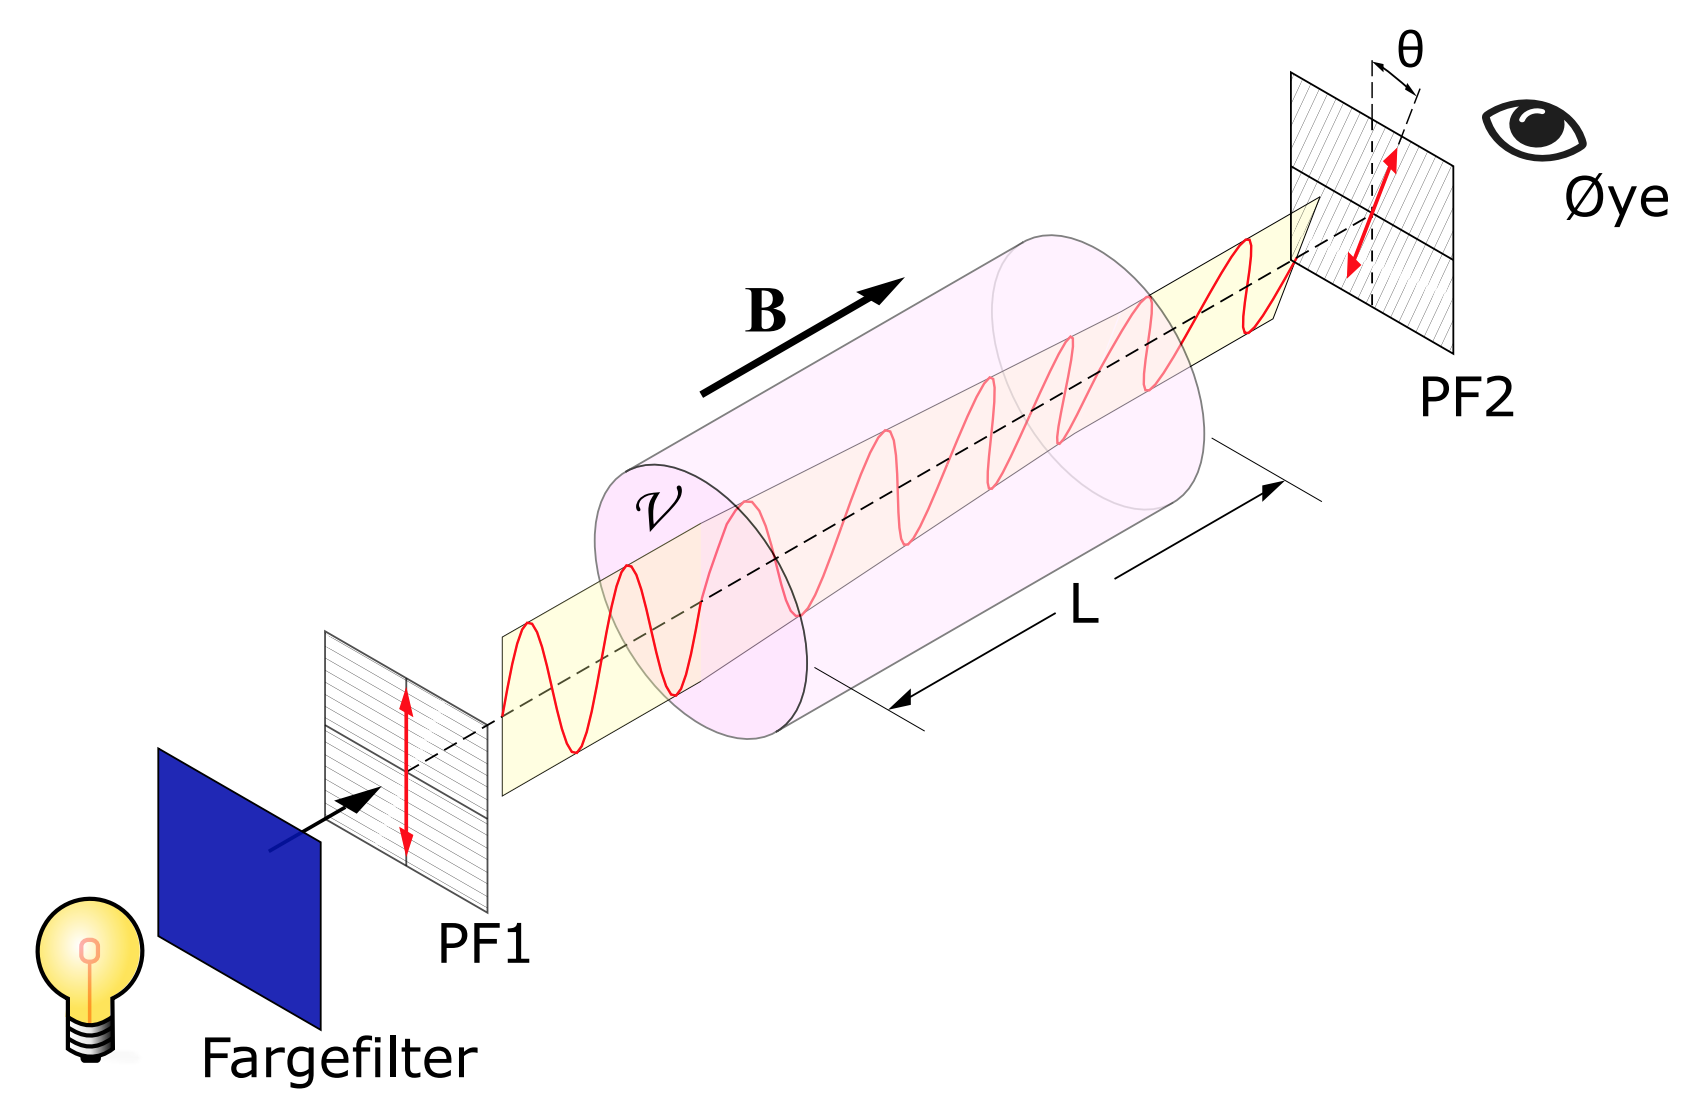
\includegraphics[scale=0.27]{oppsett3.png}
  \caption{Illustrasjon av eksperimentelt oppsett for å måle Faraday-effekten. Fra venstre til høyre i figuren ser vi lyskilden som sender lys gjennom et fargegitter, som bare slipper gjennom fotoner med ønsket bølgelengde. Bølgene som passerte gjennom fargefilteret går gjennom det første polarisasjonsfilteret, PF1. Det polariserte lyset beveger seg inn i flintglasset med lengde $L$, hvor det er et ytre magnetfelt $B$ i bevegelsesretningen til lyset. Før lyset treffer øyet må det passere gjennom det andre polarisasjonsfilteret, PF2. Ved å endre på dreiningsvinkelen $\theta$ vil en måle polarisasjonen til lyset ved å lete etter dreiningsvinkler som filtrerer ut alt lyset. Fiugren er hentet fra fysisk institutt, universitet i Oslo \cite{oppgave}.}
  \label{eksperimentelt_oppsett3}
\end{figure}
For å måle Faraday-effekten blir det brukt optiske filtere, som bare slipper gjennom noen ønskede bølgelengder, dette gjør lyset tilnærmet monokromatisk. Videre trenger vi to polarisasjonsfiltere, som plasseres på hver sin side av flintglasset. Når de to polarisasjonsfilterene står $90\degree$ på hverandre, og det ikke er noe magnetfelt, skal en ikke kunne se noe lys gjennom polarisasjonsfilteret lengst unna lyskilden. Fra å endre på styrken til magnetfeltet i flintglasset, ved å endre på strømmen som induserer magnetfeltet, ønsker vi å finne hvilken dreiningsvinkel til polarisasjonsfilteret som filtrerer alt lyset. Dette gjør vi ved å variere polarisasjonsvinkelen og se når lyset er filtrert med øyet. Eksperimentet foregår i et mørkt rom. Målingene blir gjort med magnetfeltet pekende i begge retninger, som oppstår av å sende strøm i positiv og negativ strømretning. Fra å finne forholdet mellom dreiningsvinkelen $\theta$ og styrken på magnetfeltet $B$, samt vite lengden av flintglasset $L$, kan vi beregne Verdet-konstanten fra likning \eqref{verdet}. Denne verdien kan sammenliknes med den teoretiske verdien for hver bølgelengde, som er oppgitt i databladet til utstyret brukt under eksperimentet.
I eksperimentet økte vi strømstyrken med $\SI{0.5}{\ampere}$ fra $\SI{0}{\ampere}$ til $\SI{3.0}{\ampere}$, i både positiv og negativ strømretning. Styrken på magnetfeltet inne i flintglasset er en faktor $1.5$ svakere enn styrken på magnetfeltet målt midt mellom polene.
\section{\label{sec:level4}Resultater}
\subsection{Diamagnetisme}
Ved å måle diameteren til vismutprøven på fire forskjellige punkter, fant vi at diameteren var $\SI{10.03\pm0.01}{\milli\meter}$ to steder, og $\SI{10.06\pm0.01}{\milli\meter}$. Ved å ta hensyn til spredningen i disse målingene, og usikkerheten til skyvelæret brukt, finner vi at diameteren til vismutprøven er $\SI{10.05\pm0.03}{\milli\meter}$. Dette resulterer i at tverrsnittet til vismutprøven er $\SI{79.3\pm0.2}{\milli\meter^2}$.\\
Halvparten av målingene for strøm $I$, magnetfelt mellom spolene $B_1$, magnetfelt ved toppen av vismutprøven $B_2$, og kraften på vekten $F_z$, er vist i tabell \vref{table_vismut}.
\begin{table}
  \centering
  \caption{Målinger av strøm $I$, magnetfelt mellom spolene $B_1$, magnetfelt ved toppen av vismutprøven $B_2$, og kraften på vekten $F_z$, brukt for å beregne den magnetiske susceptibiliteten til vismutprøve. Halvparten av målingene er vist i tabellen. Usikkerhetene i tabellen kommer henholdsvis fra databladet til strømgeneratoren, spredning og oppløsning til Hallsonden for måling av magnetfeltet, og databladet til vekten.}
  \label{table_vismut}
    \begin{tabular}{@{}llll@{}}\botrule
    $I$ {[}A{]} & $B_1$ {[}mT{]} & $B_2$ {[}mT{]} & $F_z$ {[}mN{]} \\ \colrule

    0.000(3)    & 18.0(3)        & 0.4(1)         & 0.0(1)      \\
    0.400(7)    & 185(2)         & 1.2(1)         & 0.2(1)      \\
    0.80(1)     & 356(4)         & 2.0(1)         & 0.6(1)      \\
    1.20(2)     & 505(5)         & 2.3(1)         & 1.3(1)        \\
    1.60(2)     & 628(6)         & 2.4(1)         & 2.0(1)        \\
    2.00(5)     & 719(7)         & 2.5(1)         & 2.6(1)        \\
    2.40(5)     & 788(8)         & 2.3(1)         & 3.0(1)        \\\botrule
    \end{tabular}
\end{table}
Målingene av den magnetiske susceptibiliteteten som funksjon av magnetfeltet mellom spolene er vist i figur \vref{resultat_chi}. Fra å gjøre en vektet midling for susceptibiliteteten over de syv målingene med høyest strøm, ved å bruke kvadratisk sammenheng mellom $B$ og $F_z$, finner vi at $\chi = -\SI{1.57\pm0.08}\cross 10^{-4}$.
Verdiene brukt for å beregne susceptibiliteteten, verdien funnet, og usikkerheten i denne verdien, er vist som et tynt blått areal i figur \vref{resultat_chi}. For å beregne susceptibiliteten har vi brukt en vektet midling under beregningen av gjennomsnittet over de siste målingene. Usikkerheten i veriden til susceptibiliteteten kommer fra usikkerheten i målingene som oppgjør susceptibiliteten \eqref{vismut}, og spredningen over susceptibiliteteten som vi ser i figuren. I figuren inkluderer det også størrelsen til susceptibiliteteten, hadde forholdet mellom den magnetiske flukstettheten og kraften på vismutprøven vært lineær \eqref{lin_chi}.
\begin{figure}[h!]
  \centering
  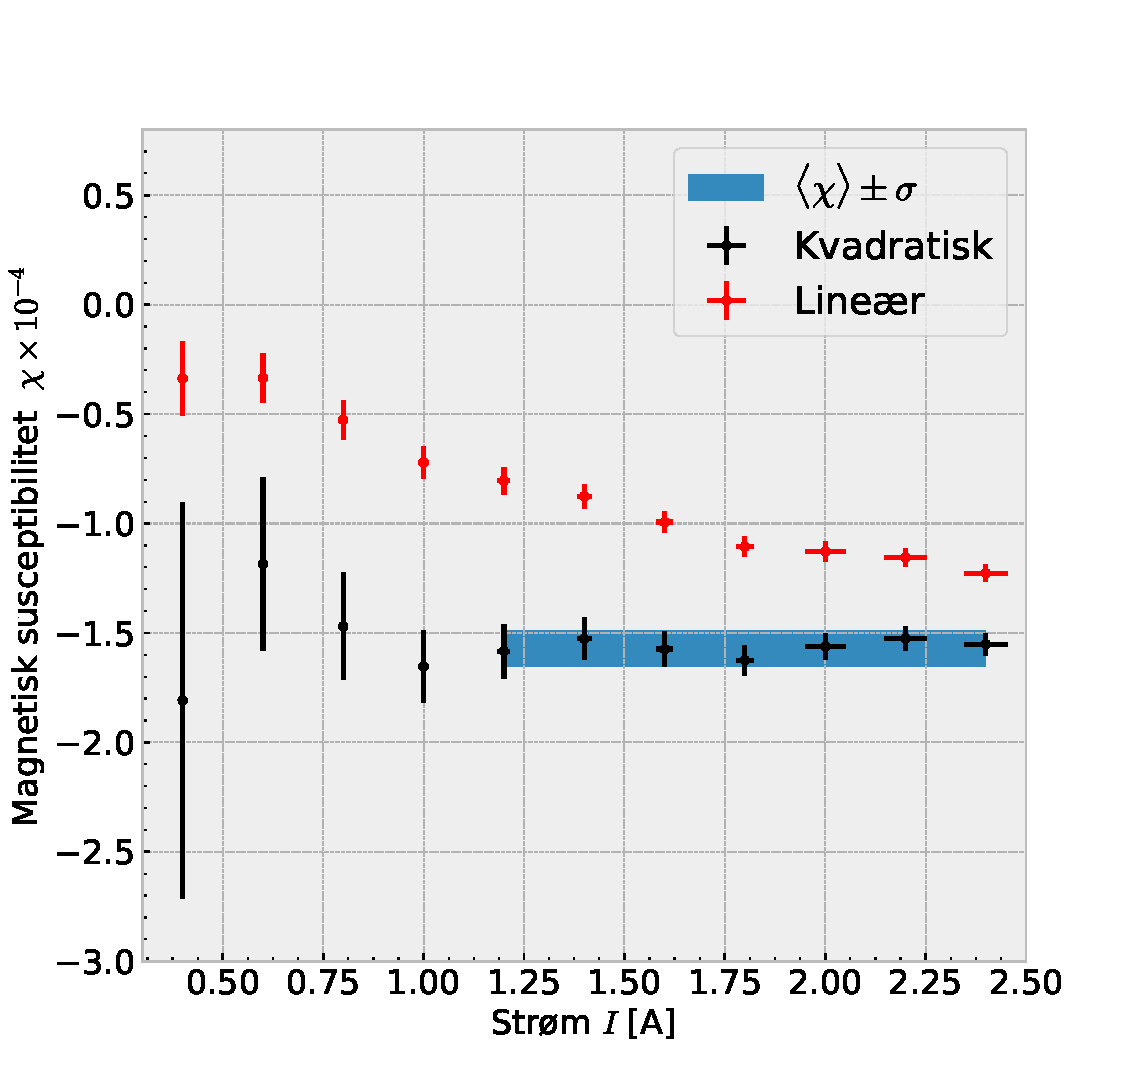
\includegraphics[scale=0.45]{chi_effekt.pdf}
  \caption{Den magnetiske susceptibiliteten $\chi$ som funksjon av strømmen $I$ i spolene. De sorte målepunktene viser susceptibiliteteten ved å bruke \eqref{vismut}, og de røde viser susceptibiliteteten ved å bruke \eqref{lin_chi}. Det blå området i grafen viser gjennomsnittet, og spredningen i gjennomsnittet, til de siste $7$ målepunktene, som viser oss at susceptibiliteteten er $\chi = -\SI{1.57\pm0.08}\cross 10^{-4}$. Gjennommsnittet er beregnet fra en vektet midling, og usikkerheten er beregnet fra usikkerheten i en enkelt måling, og usikkerheten i spredningen over gjennomsnittet.}
  \label{resultat_chi}
\end{figure}
\subsection{Ferromagnetisme}
\begin{table*}\renewcommand{\arraystretch}{1.2}
\centering
\caption{I denne tabellen er det vist de geometriske størrelsene til jernklumpene, parallelt med rotasjonsakse ($a_{\parallel}$) og tangensialt på rotasjonsaksen ($a_{\perp}$). Fra disse målingene kan en beregne avmagnetiseringsfaktoren parallelt med magnetfeltet ($D_{\parallel}$) og tangensialt på magnetfeltet ($D_{\perp}$). Usikkerheten til målingene kommer fra usikkerheten til skyvelæret. Videre i tabellen vises styrken til magnetfeltet i kontakt med jernklumpen, når rotasjonsaksen til jernklumpen er parallell med magnetfeltet ($B\parallell$) og tangensialt på magnetfeltet ($B\perp$). Usikkerheten er beregnet fra databladet til hallsonden. For å teste teorien \eqref{upper_limit} inkluderer tabellen $B_0/D_i$, som indikerer øvre grense for $B_i$, hvor $i$ enten indikerer parallell $\parallel$ eller ortogonalt $\perp$.}
\label{tot_ferro}
\begin{tabular}{@{}lllllllll@{}}
\botrule
Form & $a_{\parallel}$ {[}cm{]} $\quad$  & $a_{\perp}$ {[}cm{]} $\quad$  & $D_{\parallel}$ $\qquad \quad$ & $D_{\perp}$ $\qquad\quad$ &  $\bm{B}$  $\parallel$ {[}mT{]} $\quad$ & $\bm{B}$ $\perp$ {[}mT{]} $\quad$ & $B_0/D_{\parallel}$ [mT]$\quad$  & $B_0/D_{\perp}$ [mT]\\ \colrule

Skive      & 0.67(1)        & 5.99(2)           & 0.99(8)         & 0.005(4) & 5.50(1)                           & 17.58(4)         &    5.1(4)  &  1036(86)      \\
Ellipsoide & 21.8(2)        & 0.96(1)           & 0.055(8)        & 0.50(5) & 50.5(1)                           & -                &   920(80)    & 10.1(8)       \\
Sylinder   & 6.45(2)        & 0.98(1)           & 0.037(3)        & 0.48(4) & 19.65(4)                          & 7.74(2)          &   133(11)    &10.5(9)           \\
Kule       & 6.32(2)        & 6.32(2)           & 0.33(3)         & 0.33(3) & 12.61(3)            & 12.61(3)                &   15(1)  & 15(1)        \\ \botrule
\end{tabular}
\end{table*}
Vi ønsker nå å studere de magnetiske egenskapene til jern ved å måle styrken på magnetfeltet, mens jernklumpen er plassert i en spole. For å sammenlikne resultatene med teori trenger vi de geometriske størrelsene til de fire jernklumpene vi skal se på. Det ble derfor gjennomført målinger av diameter og høyde med et skyvelær, resultatene er vist  i tabell \vref{tot_ferro}.
Ved å sende en konstant strøm på $\SI{5}{\ampere}$ i sløyfen generes det et magnetfelt inne i spolen. Vi målte styrken til strømmen med et multimeter til å være $\SI{5.00\pm0.01}{\ampere}$. Videre bruker vi en Hallsonde til å måle styrken på magnetfeltet, over flere målinger finner vi at styrken på magnetfeltet er $\SI{5.04\pm0.04}{\milli\tesla}$, usikkerheten kommer fra spredningen i målingene. Magnetfeltet er ikke homogent i hele spolen. Magnetfeltet høyere i spolen, men i det radielle sentrum, var $\SI{2.6\pm0.1}{\milli\tesla}$. I midten av spolens høyde måler vi at magnetfeltet er $\SI{4.8\pm0.1}{\milli\tesla}$ halvveis radielt ut mot spolen, og $\SI{4.7\pm0.1}{\milli\tesla}$ helt i kanten av spolen. Usikkerhetene kommer fra databladet til Hallsonden.\\
Deretter ble det målt styrken på magnetfeltet med plastikkstativet inne i spolen. Endringen i styrken på magnetfeltet var innenfor usikkerheten til magnetfeltet. Plastikkstativet påvirker altså ikke magnetfeltet inne i spolen. \\
De fire jernklumpene ble plassert på plastikkstativet, inne i spolen, med strømmen på. Ved å måle styrken på magnetfeltet på overflaten til jernklumpen med Hallsonden rettet parallelt med feltet, fikk vi målingene vist i tabell \vref{tot_ferro}.\par
Vi kan også studere magnetfeltet rundt en jernklump ved å se på hysteresekurver. Under eksperimentet ble det brukt en sekundærspole med $n=135$ vindinger, og en diameteren på $\SI{6.5pm0.1}{\milli\meter}$, som gjør at arealet er $\SI{33\pm1}{\milli\meter^2}$. Kalibreringskonstanten $\kappa$ til spenningsgeneratoren var oppgitt til å være $\SI{1.01}{\micro\weber}$. Fra disse verdiene kan vi beregne endringen i magnetfelt fra likning \eqref{deltas}, det eneste som mangler er $\Delta S$. Integralet fra spennignsgeneratoren $\Delta S$, målt av spenningsintegratoren, ble vist på datamaskinen som en funksjon av strømmen i sekundærspolen. Det eneste som trengte å endres var maksimalstyrken på strømmen $I$ i primærspolen. Fra å studere magnetiseringen av jernsylinderen før vi sende strøm i spolen målte vi at jernet var magnetisert, i positiv retning. Initialtilstanden til jernet var magnetisert. Styrken på magnetfeltet inne i sekundærspolen blir regnet ut ved likning \eqref{deltab}, og er vist som en funksjon av strømmen i sekundærspolen i figur \vref{data_delta_B}.
\begin{figure}[h!]
  \centering
  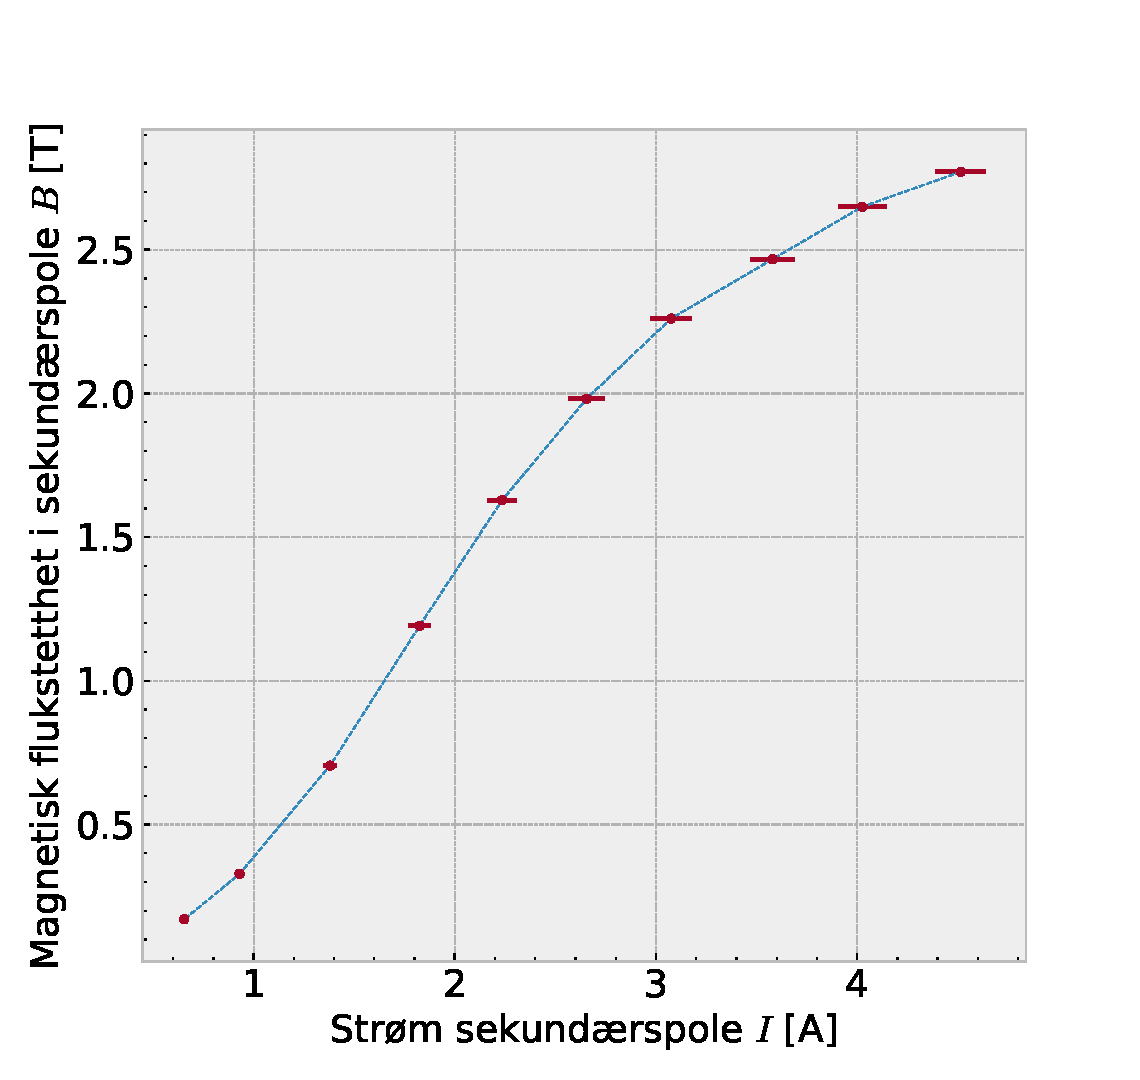
\includegraphics[scale=0.45]{magnetic_secondary_hysterese.pdf}
  \caption{Styrken på det magnetiske feltet inne i sekundærspolen som funksjon av strømmen i sekundærspolen, som er indusert av strømmen i primærspolen. I figuren ser vi at det ikke er en lineær sammenheng mellom styrken på strømmen, og styrken på magnetfeltet.}
  \label{data_delta_B}
\end{figure}
Et eksempel på målingene som utgjorde en hysteresekurve er vist i figur \vref{hysterese}, hvor vi ser spenningsintegratorens verdi $S$ som en funksjon av strøm i sekundærspolen. Fra målinger, som den vist i figur \vref{hysthyst}, kunne vi beregne den magnetiske flukstettheten $B$ for en verdi av strømmen i primærspolen, og måtte gjentas for forskjellige strømstyrker, som ga oss målingene vist i figur \vref{delta_delta_B}.
\begin{figure}[h!]
  \centering
  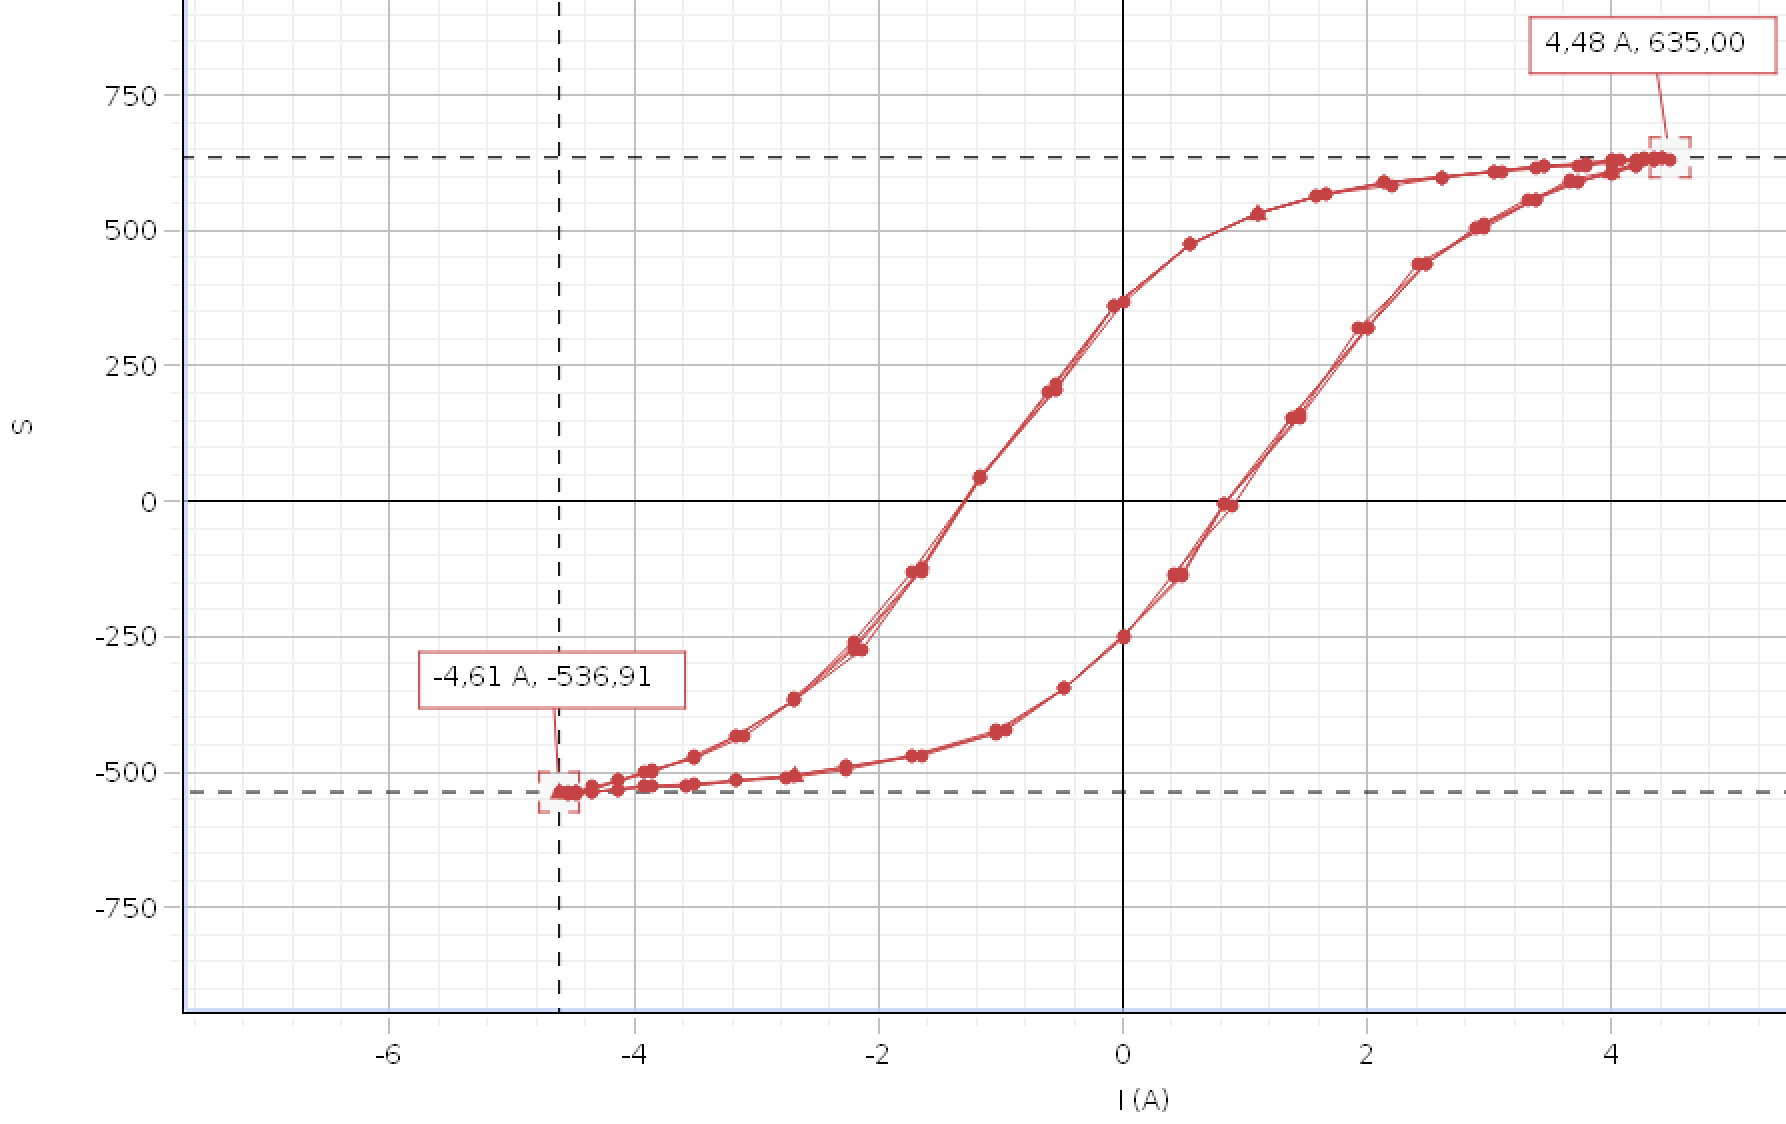
\includegraphics[scale=0.25]{Hysterese.png}
  \caption{Målinger av spenningsintegratorens verdi som funksjon strøm i sekundærspolen over tid. Kurven gjentar seg selv flere ganger. Denne kurven er ett eksempel på en måling for en bestemt verdi i primærspolen, og målinger som denne ble gjentatt flere ganger for forskjellig strømstyrk.e}
  \label{hysthyst}
\end{figure}
Fra å vite størrelsen på strømmen i primærspolen kan vi beregne magnetiseringen av jernstangen, som sekundærspolen er tvinnet rundt. Magnetiseringen ønsker vi å vite som en funksjon av den ytre påtrykte strømmen $H_0$, som vi kan beregne fra \eqref{nice_H}. Vi har all informasjon til å beregne $H_0$, og vi har målingene for styrken på magnetfeltet $B$, som gjør at magnetiseringen kan beregnes ved likning \eqref{get_H}. Forholdet mellom magnetiseirngen $M$ og $H$-feltet grunnet strømmen i spolen er vist i figur \vref{MH0}.
\begin{figure}[h!]
  \centering
  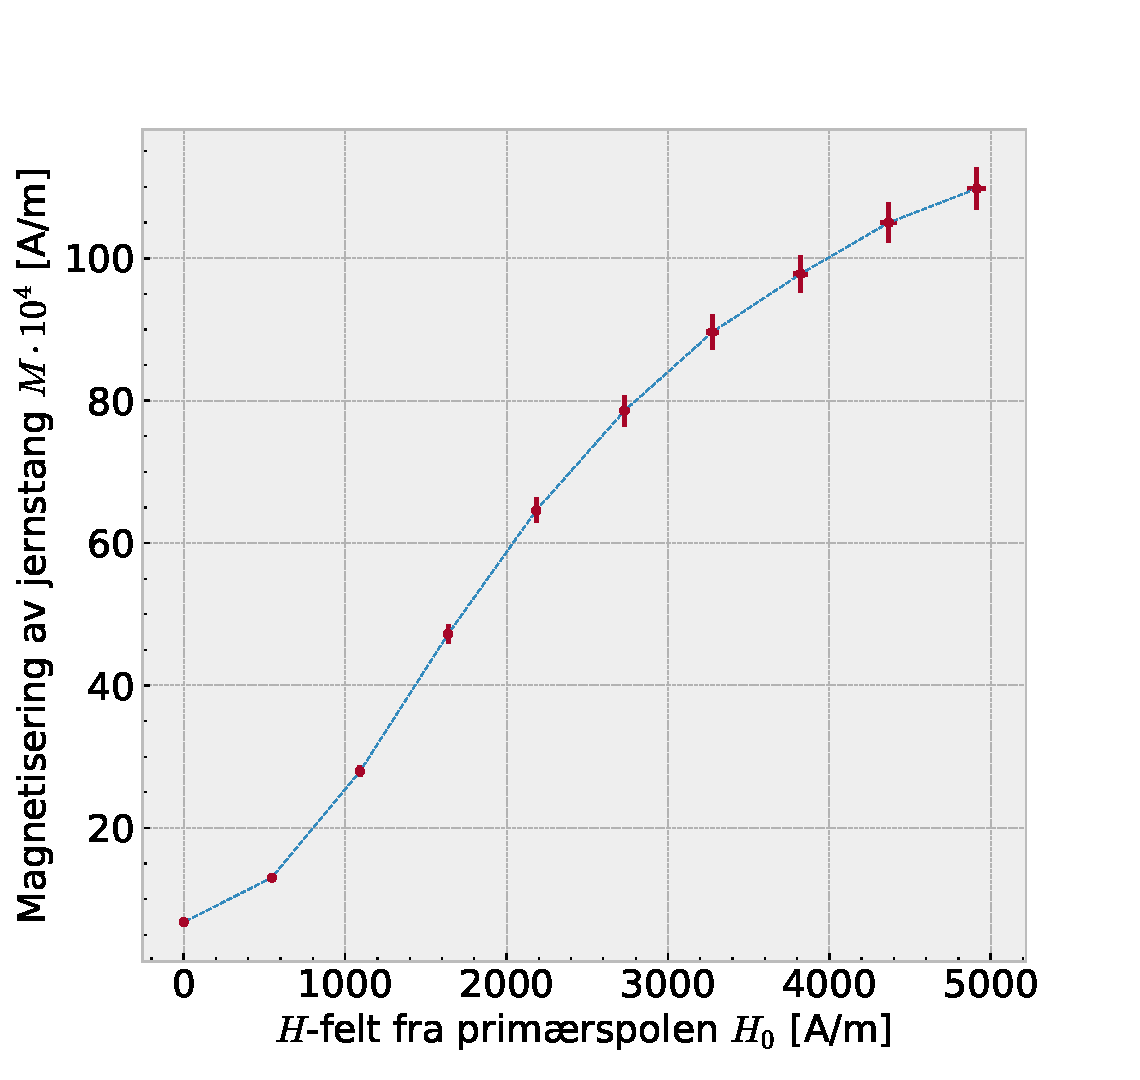
\includegraphics[scale=0.45]{magnetisering.pdf}
  \caption{Magnetiseringen av jernsylinderen, med sekundærspolen tvunnet rundt, som en funksjon av $H$-feltet generert av primærspolen. Den rette linjen viser oss at det ikke er et lineært forhold mellom magnetiseringen og $H_0$. Merk også at denne figuren har samme form som styrken på magnetfeltet vist i fiugr \vref{data_delta_B}.}
  \label{MH0}
\end{figure}
\subsection{Faraday-effekten}
For å beregne Verdet-konstanten ble det gjennomført målinger av polarisasjonsgraden til lys som funksjon av styrken på det ytre magnetfeltet. Disse målingene er vist i tabell \vref{faraday}. Styrken på magnetfeltet avtar med en faktor $1.5$ inne i flintglasset, dette er tatt hensyn til i tabellen, og under beregningen av stigningstallet. Fra å beregne stigningstallet til polarisasjonsvinkelen som funksjon av produktet mellom magnetfeltet og lengden på flintglasset \eqref{verdet} kunne vi beregne Verdet-konstanten. Verdien til Verdetkonstanten er vist, for de tre forskjellige bølgelengdene brukt under eksperimentet, i tabell \vref{faraday}.
\begin{table}\renewcommand{\arraystretch}{1.1}
  \centering
  \caption{I denne tabellen er det vist målt vinkel for $\theta [\degree]$, for forskjellig styrke i magnetfelt, for begge strømretninger. Usikkerheten i vinkelen er lik $0.3\degree$ for alle målinger. Styrken på magnetfeltet vist i tabellen, er styrken inne i flintglasset. Fortegnet til vinkelen forteller oss om retningen på strømmen er positiv eller negativ. Nederest i tabellen er det beregnet stigningstall for målepunktene i både negativ og positiv strømretning for hver bølgelengde. Usikkerheten i stigningstallet kommer av lineærregresjonen \cite{squires}.}
  \label{faraday}
  \begin{tabular}{|l|S|S|S|S|S|S|}
    \colrule
      Bølgelengde $\lambda$ [nm] &
      \multicolumn{2}{|c|}{$440$} &
      \multicolumn{2}{c|}{$580$} &
      \multicolumn{2}{c|}{$595$} \\
      \colrule

      $B$ [mT] & \multicolumn{6}{c|}{Vinkel $\theta\pm0.3$ [$\degree$] } \\   \colrule

      43(1)  & 1.8 & -1.4 & 1.8 & -1.4 & 2.0 & -1.6 \\
      63(1)  & 2.8 & -2.2 & 2.6 & -2.0 & 2.8 & -2.6 \\
      83(1)  & 3.8 & -3.0 & 3.0 & -2.8 & 3.6 & -3.2 \\
      102(2) & 4.2 & -4.0 & 4.0 & -3.4 & 4.4 & -4.2 \\
      119(2) & 5.2 & -4.8 & 4.4 & -4.0 & 5.2 & -4.8 \\ \colrule

      Stigningstall [da$\degree$/Tm] &
      \multicolumn{2}{|c}{$135(2)$} &
      \multicolumn{2}{|c}{$140(1)$} &
      \multicolumn{2}{|c|}{$119(1)$} \\
      \colrule
  \end{tabular}
\end{table}
Målingene er også vist grafisk i figur \vref{fig_verdet}. Figuren viser polarisasjonsvinkel $\theta$ som funksjon av produktet mellom magnetfeltet og lengden på flintkrystallen. Stigningstallet til linjene i denne figuren tilsvarer Verdet-konstanten.
\begin{figure}[ht!]
  \centering
  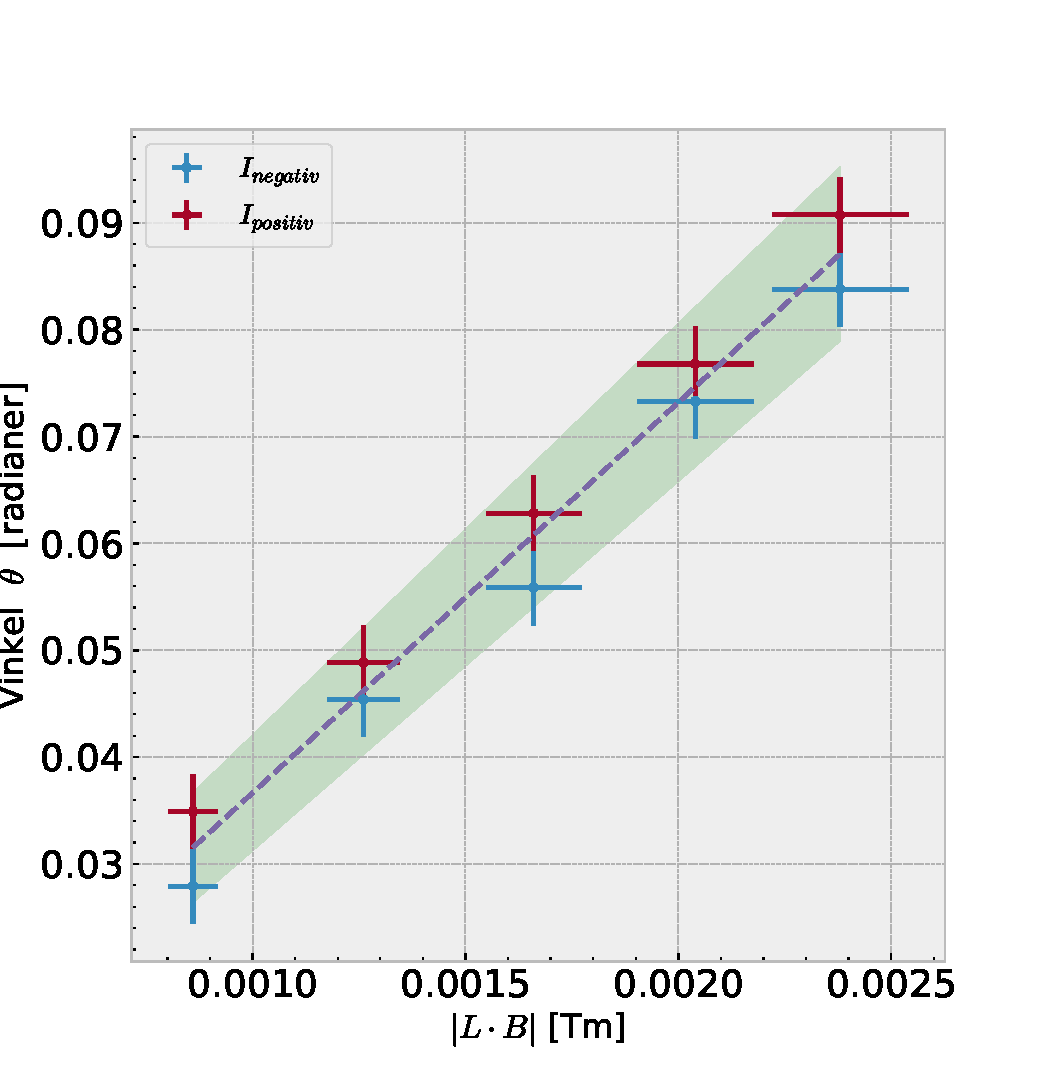
\includegraphics[scale=0.45]{faraday_effekt.pdf}
  \caption{Målinger for polarisasjonsvinkel $\theta$ som funksjon av produktet mellom styrken til magnetfeltet og lengden av flintkrystallen, for alle bølgelengdene brukt under eksperimentet. Fra målepunktene beregnes stigningstallet ved hjelp av lineærregresjon for hver bølgelengde, som gir oss Verdet-konstanten. Verdien til hvert målepunkt er tydeligere vist i tabell \vref{faraday}.}
  \label{fig_verdet}
\end{figure}
Resultatene viser oss Verdet-konstanten for de $3$ forskjellige bølgelengdene er: $\lambda = \SI{440}{\nano\meter}$ $\SI{135\pm2}{\deca\degree/\tesla\meter}$, $\lambda = \SI{580}{\nano\meter}$ $\SI{140\pm1}{\deca\degree/\tesla\meter}$, og $\lambda = \SI{595}{\nano\meter}$,
 og $\SI{119\pm1}{\deca\degree/\tesla\meter}$. Hvor usikkerheten er beregnet fra usikkerheten i stigningstallet fra lineærregresjonen \cite{squires}.
\section{Diskusjon}
\subsection{Diamagnetisme}
Verdiene brukt for å beregne den magnetiske susceptibiliteteten er vist i figur \vref{resultat_chi}. Som vi ser i figuren avtar usikkerheten som styrken på strømmen øker. Dette er fordi den relative usikkerheten til vekten er stor når utslaget på vekten er lite, siden usikkerheten er konstant $\SI{0.01}{\gram}$. For å beregne verdien til $\chi$ bruker vi derfor en vektet midling på de $7$ siste punktene. Målingene med høyere usikkerhet blir vektet lavere i beregningen av gjennomsnittet, for de siste $7$ målingene. Dette resulterte i at verdien til susceptibiliteteten ble $\chi = -\SI{1.57\pm0.08}\cross 10^{-4}$. Vektingen er slik at målinger med høy usikkerhet teller mindre i gjennomsnittet, som eksempel teller målepunktet for $I=\SI{2.4}{\ampere}$ en faktor 4 mer i beregningen av gjennomsnittet, i forhold til målepunktet for $I=\SI{1.2}{\ampere}$ i beregningen av usikkerheten. Usikkerheten til susceptibiliteteten kommer av spredningen til målingene brukt, og usikkerheten til hver enkelt måling.\par
I tabell \vref{table_vismut} er målingene gjort for å beregne den magnetiske susceptibiliteteten vist. Fra verdiene ser vi at kraften som virker på vismutstangen øker med styrken på magnetfeltet. Som strømmen i spolene øker, øker kraften på den magnetiske flukstettheten. Den magnetiske flukstettheten mellom spolene $B_1$ øker nesten lineært med strømstyrken, men mot slutten avtar stigningen svakt. Styrken på magnetfeltet på den andre enden av staven går mot en konstant verdi på rundt $\SI{2.4}{\milli\tesla}$, når strømmen når $\SI{1.20}{\ampere}$. Fra å bruke likning \eqref{test_chi} kan vi teste effekten av å sette $B_2=\SI{0}{\tesla}$. Verdien til $\chi$ blir mer nøyaktig, jo sterke magnetfeltet er, vi bruker derfor verdien til den magnetiske flukstettheten for strømmen $I=\SI{2.4}{\ampere}$. Dette gir oss en endring av $\chi$
på $2.161(7)\cross10^{-9}$, som tilsvarer en prosent endring på $0.000138(4)\%$. Altså har det ingen effekt ved å inkludere $B_2$ i beregningen av susceptibiliteteten. Faktisk vil økningen av usikkerheten til susceptibiliteteten øke med $\SI{4.11}\cross 10^{-8}$ om en inkludere $B_2$ i beregningen. Denne usikkerheten er den midlede usikkerheten for de siste $7$ målepunktene. Økningen av usikkerheten til susceptibiliteteten vil være større enn økningen av susceptibiliteteten. Det vil derfor gi mer presise resultater ved å ikke inkludere $B_2$, enn å gjøre det, selv om dette er nærmere det analytiske uttrykket. \\
I figur \vref{resultat_chi} vises også susceptibiliteteten om vi hadde antatt et lineært forhold mellom magnetfeltet og kraften i likning \eqref{vismut}. Dette ville gjort at susceptibiliteteten er gitt av likning \eqref{lin_chi}. Som vi ser i figuren er dette ikke en god tilnærming. Av å sammenlikne susceptibiliteteten målt i dette eksperimentet med andre målinger, fant vi at vår verdi var litt for høy, men ganske nære. Hadde vi antatt et lineært forhold mellom magnetfeltet og kraften ville avviket vært enda større fra den korrekte verdien til susceptibiliteten. Det er ikke en god antagelse å anta lineært forhold mellom kraften $F_z$ og magnetfeltet $B$. Itillegg ser vi at verdien for susceptibiliteten ved å anta et lineært forhold ikke går mot en konstant verdi som strømmen øker. Ved å anta lineært forhold vil verdien til susceptibiliteteten være avtagende for alle målepunktene brukt under dette eksperimentet. Dette kan vises ved at stigningstallet til målepunktene, vist i figur \vref{resultat_chi}, for de siste syv målepunktene er $\SI{-3.5(3)e-5}{\per\ampere}$ ved å anta lineært forhold, og $\SI{2(3)e-06}{\per\ampere}$ ved å anta kvadratisk forhold. Altså er stigningstallet samme størrelsesorden som susceptibiliteteten ved å anta lineært forhold, mens ved å anta et kvadratisk forhold er stigningstallet rundt en faktor $10$ lavere. Det vil si at susceptibiliteten flater ut mot en konstant verdi for det kvadratiske forholdet, men avtar lineært for det lineære forholdet.
I et framtidig eksperiment hadde det vært ønskelig å studere den lineære antagelsen videre, for høyere strømmer, og se nøyere på hvordan forholdet mellom det lineære og kvadratiske uttrykket utvikler seg. Siden utledning fra Maxwell's likninger viser at det skal være et kvadratisk forhold mellom den magnetiske kraften og styrken på magnetfeltet gir det mening at det kvadratiske uttrykket gir bedre overenstemmelse med andres målinger av den magnetiske susceptibiliteteten.
\par
Den magnetiske susceptibiliteteten ble målt til å være $-\SI{1.57\pm0.08}\cross 10^{-4}$. Denne verdien kan vi teste mot andres målinger av den samme veriden. susceptibiliteteten til vismut funnet i tabeller (\cite{noauthor_magnetic_2018} \cite{noauthor_magnetic_nodate}) er $-1.66 \cross 10^{-4}$.
Det er derfor et avvik på $0.001$ mellom den målte verdien av susceptibiliteteten og verdien funnet i tabeller, ved å ta med usikkerheten. Dette innebærer et avvik på $0.6\%$ mellom den målte verdien, og den funnet i tabeller. Avviket er lite, men kan ha vært forårsaket av en systematisk feil under eksperimentet. Under eksperimentet prøvde vi å plassere vismutstaven midt mellom spolene, slik at det ble utsatt for kraftigst mulig magnetfelt. Vi passet på at vismutprøven ikke hvilte inntil spolene, eller var i kontakt med noe annet, som kunne forårsaket friksjon, som ville gitt et utslag på vekten, men det kan ha skjedd under eksperimentet likevel. Det gikk også en tid mellom den magnetiske flukstettheten mellom spolene ble målt, og vismutprøven ble utsatt for feltet. Magnetfeltet kan ha forandret seg iløpet av denne tiden, eller målingen vår med Hallsonden ikke var stødig nok. Dette er noen eksempler på systematiske feil som kan ha forårsaket avvik mellom verdien vi målte for susceptibiliteteten, og verdien funnet i tabeller. Itillegg er susceptibiliteteten temperaturavhengig, og temperaturen brukt når susceptibiliteteten var funnet i tabellene var ikke nødvendigvis den samme brukt under vårt eksperiment.
\subsection{Ferromagnetisme}
Før målingene ble gjennomført med jern i sentrum av spolen målte vi magnetfeltet i spolen. I sentrum av spolen, både radielt og i høyde, var den magnetiske flukstettheten tilnærmet konstant. Spredningen i målingene var samme størrelsesorden som usikkerheten med Hallsonden. Vi målte at den magnetiske flukstettheten var $\SI{5.04\pm0.4}{\milli\tesla}$, denne verdien kan vi sammenlikne med den teoretisk forventede verdien fra likning \eqref{nice_b}. Spolen brukt under eksperimentet var $\SI{275}{\milli\meter}$ lang, og var vindet $244$ ganger rundt. Ved å bruke naturkonstanten $\mu_0 = \SI{4\pi e-7}{\tesla\meter/\ampere}$ betyr dette at den forventede styrken på magnetfeltet er $\SI{5.57\pm0.01}{\milli\tesla}$. Det blir målt en lavere styrke på magnetfeltet enn den teorien forutsier. En årsak til dette kan være at det ikke blir brukt idelle ledninger under eksperimentet. I en spole må en velge mellom en høy induktans eller en lav motstand, siden hensikten med denne spolen er å generere et magnetfelt, er det mulig at det er en stor motstand i ledningene. Dette er noe som burde vært målt med et multimeter under eksperimentet. Den teoretiske størrelsen til magnetfeltet tar ikke hensyn til motstand i ledningene, og dette kan være grunnen til avviket med den eksperimentelt målte verdien.\\
Under eksperimentet ble det gjennomført målinger om hvorvidt stativet å sette jernklumpene på påvirket magnetfeltet. Vi fant at stativet ikke hadde noen påvirkning på magnetfeltet. Ved å sjekke susceptibiliteten til plastikk, som stativene var laget av, i tabeller \cite{plastikk_sucept}, finner vi at susceptibiliteteten er tilnærmet lik $0$. Dette betyr at plastikk som blir påtrykket av et ytre magnetisk felt, som vi gjorde under dette eksperimentet, ikke vil påvirke styrken på magnetfeltet. Styrken vil være tilnærmet den samme, og det var akkurat dette vi målte på eksperimentet. Vi trenger altså ikke å ta hensyn til effekten av plastikkstativet ved analyse av målingene.\\
Målingene gjort for de fire forskjellige jernklumpene er vist i tabell \vref{tot_ferro}. Denne tabellen inkluderer målingene av lengden til de fire jernklumpene, parallelt med, og tangensialt på, symmetriaksen.
Fra tabellen ser vi at lengden til ellipsoiden parallelt med symmetriaksen har en faktor tre større relativ usikkerhet enn de andre lengdene. Årsaken til dette er at dette målet måtte bli gjort med en meterstokk istedenfor et skyvelær, som fører til en større usikkerhet. Denne usikkerheten manifesterer seg ikke merkbart i de følgende usikkerhetene for ellipsoiden. Fra lengden til jernklumpene kunne vi beregne avmagnetiseringsfaktoren til jernklumpen parallelt med, og ortogonalt på rotasjonsaksen. Disse brukes til å finne den øvre grensen for magnetfeltet når symmetriaksen til jerklumpen er plassert henholdsvis parallelt med og ortogonalt på magnetfeltet, ved likning \eqref{upper_limit}. Som vi ser fra verdiene i tabellen tilfredstiller den målte verdien til den magnetiske flukstettheten den øvre grensen som teorien forutsier, for alle formene, i begge retninger.\\
Under eksperimentet ble det brukt en skive og en sylinder, teorien forutsetter at de geometriske formene til jernklumpene er ellipsoider. Både sylinderen og skiven er ikke ellipsoider, men blir tilnærmet som det under eksperimentet. Dette er en grov tilnærming, men som vi ser fra resultatene stemte de fortsatt med teorien. For den skiveformede jernmagneten ble ikke ulikheten i likning \eqref{upper_limit} tilfredstilt uten å ta hensyn til måleusikkerheten. Ved å beregne differansen mellom $B\parallel$ og $B_0/D_{\parallel}$ og usikkerheten i differansen \eqref{usikk2}, får vi at differansen er $\SI{0.4\pm0.41}{\milli\tesla}$, altså er ulikheten i likning \eqref{usikk1} tilfredstilt, det er overensstemmelse innenfor måleusikkerhetene.\\
Vi kan teste verdiene funnet for avmagnetiseringsfaktoren ved å sammenlikne verdien med avmagnetiseringsfaktoren for kjente ellipsoider. For en kule vil avmagnetiseringsfaktoren være $1/3$ parallelt og tangensialt på, dette stemmer med de vi har målt. For flate skiver går $D_{\parallel}$ mot $1$, og $D_{\perp}$ mot $0$. Dette ser vi stemmer for skiven, siden den ikke er fullstendig flatklemt. For høyere og smalere ellipsoider går $D_{\parallel}$ mot $0$, og $D_{\perp}$ mot $1/2$. Dette ser vi stemmer godt overens for ellipsoiden, og litt mindre godt for sylinderen, som er litt bredere, og litt lavere.
\par
Fra å genere en varierende spenning, og bruke Faradays induksjonslov \eqref{3}, kunne vi beregne styrken på magnetfeltet ved å måle strømmen i spolen. Jern er en ferromagnet, og dette ser vi fra det ikke-lineære forholdet mellom strømmen i sekundærspolen og styrken på magnetfeltet, vist i figur \vref{data_delta_B}. Her ser vi tydelig at susceptibiliteten er en funksjon av det påtrykte magnetfeltet. Studerer vi nærmere magnetiseringen til en jernstang som en funksjon av strømmen i den ytre spolen, vist i figur \vref{MH0}, ser vi en annen egenskap ved ferromagneter, det magnetiske feltet blir forsterket med en veldig stor forsterkning. Dette ser vi fra at magnetiseringen til jernet er omtrent en faktor $500$ større enn $H$-feltet generert fra primærspolen. Dette er årsaken til at kurvene i figur \vref{data_delta_B} og figur \vref{MH0} har lik form, bidraget til magnetfeltet fra spolen er så lite iforhold til bidraget fra jernsylinderen som blir magnetisert, at det blir en liten forskjell i formen på kurvene. Det er akkurat dette vi forventer av ferromagnetiske materialer.\\
Fra figur \vref{MH0} ser vi at magnetiseringen av jernet øker med $H_0$. Men denne økningen avtar for høye verdier for $H_0$, fra målingene ser det ut som at magnetiseringen av jernet går mot en maksimal magnetisering. Når størrelsen på magnetfeltet generert av primærspolen når en verdi, vil det ikke klare å magnetisere materialet ytterligere, og det er dette vi ser fra målingene. Dette er forventet for ferromagneter, retningen til angulærmomentet av elektronbanene vil ikke rette seg inn noe mer av en økning i feltstyrken utenfor materialet. Utover dette har vi ingen enkel teori å sammenlikne magnetiseringen med. For ferromagneter er det et komplekst forhold mellom det ytre magnetiske feltet og magnetiseringen. Magnetiseringen er avhengig av både geometri, material og feltstyrken.
\subsection{Faraday-effekten}
Målingene av vinkel som funksjon av magnetfelt er vist i tabll \vref{faraday}. I denne tabellen er polariseringsvinkelen vist for både positiv og negativ strømretning. Som vi ser fra tabellen er polarisasjonsgraden når strømretningen er negativ konsekvent lavere enn når strømretningen er positiv, for alle målingene. Ifølge teorien burde polarisasjonsvinkelen være uavhengig av retningen til $B$-feltet. Hva kan isåfall forårsake denne systematiske forskjellen av polariseringen? En mulighet kan være at flintglasset blir magnetisert, og denne magnetiseringen sitter igjen når magnetfeltet endrer retningen. Fra produsenten av flintglasset er det oppgitt at styrken på magnetfeltet avtar med en faktor $1.5$ i flintglasset, men at retningen på magnetfeltet ikke skal ha noen innvirkning på måleresultatene. Dette kan derfor ikke være årsaken til avviket mellom polarisasjonsvinkel for de to strømretningene. Retningen til $B$-feltet vil i begge tilfeller være rettet parallelt med rotasjonsaksen til flintglasset, så aksen til flintglasset i magnetfeltet burde ikke ha noen påvirkning, siden den er lik for forskjellig strømretning. Fargefilteret, og polarisasjonsfilterene er langt nok ute av magnetfeltet til at disse ikke vil bli påvirket av magnetfeltet. En annen grunn kan være at polarisasjonsvinkelen for $B=\SI{0}{\tesla}$ ble feilvalgt under eksperimentet, og at denne posisjonen burde vært forskjøvet $0.2-0.4\degree$ i positiv retning. Dette ville gjort at polariseringen av lyset ville vært nærmere hverandre for de to strømretningene. Heldigvis vil en feilvalgt verdi for null-punktet ikke ha en innvirkning på stigningstallet, altså Verdet-konstanten, siden dette kunn avgjør konstantleddet i lineærregresjonen.\\
%Noe annet å merke seg er at for $\lambda=\SI{440}{\nano\meter}$ er alle målingene, i absoluttverdi, større enn sine tilsvarende målinger for $\lambda=\SI{580}{\nano\meter}$. En ville da forvente at når bølgelengden er  $\SI{595}{\nano\meter}$ vil verdiene fortsette å være lavere enn for $\lambda = \SI{440}{\nano\meter}$, muligens en litt større forskjell. Men det er ikke dette vi observerer i tabell \vref{faraday} og figur \vref{fig_verdet}.
%For denne bølgelengden er polarisasjonsvinkelen nærmere polarisasjonsvinkelen når bølgelengden var $\lambda=\SI{440}{\nano\meter}$, og av og til større, i absolutt verdi. Dette forventet vi ikke.
Målingene funnet for Verdet-konstanten kan sammenliknes med den teoretisk forventede verdien, som er oppgitt i databladet. Der finner vi at Verdetkonstanten er $2857, 1428, \SI{1210}{\degree/\tesla\meter}$, henholdsvis for bølgelengdene $440, 580, \SI{595}{\nano\meter}$. Disse verdiene tyder på at det har skjedde en systematisk feil under målingene for lys med bølgelengde på $\SI{440}{\nano\meter}$. For lys med bølgelengde $\SI{480}{\nano\meter}$ er det et avvik på $2(1)\%$, for lys med bølgelengde på $\SI{595}{\nano\meter}$ er det et avvik på $1(1)\%$. Dette er et lite avvik fra den forventede verdien. Avviket kan komme av tilfeldige feil som det ikke har blitt tatt hensyn til under beregningen av usikkerheten. Itillegg er ikke usikkerheten i hvert målepunkt tatt med i betraktningen for usikkerheten i stigningstallet. Under beregningen av usikkerheten i stigningstallet ble det ikke tatt hensyn til usikkerheten i hver enkelt måling, dette har gjort usikkerheten i stigningstallet lavere enn den egentlig skal være. Forandringen ville ikke vært avgjørende, siden det er den lineære økningen vi er interesert i, men en burde merke seg at usikkerheten i vinkelen, relativt til differansen mellom to vinkler, er høy.
For Verdetkonstanten med bølgelengde på $\SI{440}{\nano\meter}$ er det et ekstremt avvik mellom den eksperimentelle, og verdien fra databladet, avviket er på hele $47.4(8)\%$. Et avvik av størrelsesorden faktor $2$ kommer av systematiske feil under eksperimentet. Siden et så stort avvik kunn opsto for denne bølgelengden kan avviket komme av en systematisk feil i gitteret brukt under eksperimentet, siden dette er den eneste delen av eksperimentet som forandret seg for målinger av forskjellig bølgelengder. Det er mulig det er noen hull i teorien verdien blir testet mot, men avviket stammer mest sansynlig av en systematisk feil gjort under eksperimentet. Under fremtidige eksperimenter burde derfor Verdet-konstanten for denne bølgelengden studeres nærmere.
Måleapparatet for polarisasjonsvinkelen har en oppløsning på $0.2\degree$, følgelig vil verdiene målt ikke kunne være mer presise enn $0.2\degree$. Intervallet av vinkler vi måler under eksperimentet er mellom $1.4$ til $5.2\degree$, med en økning på rundt $1\degree$ mellom hvert målepunkt. For denne endringen av vinkelen mellom hvert målepunkt, er en oppløsning på $0.2\degree$ ikke ideelt. Dette ser vi tydelig i figur \vref{fig_verdet}, hvor målepunktene ofte er på samme verdi, eller at usikkerheten i ett målepunkt overlapper med usikkerheten for et annet målepunkt. For lys med bølgelengde på $\SI{440}{\nano\meter}$ var det det en systematisk feil tilstedet under eksperimentet, og målingene burde tolkes deretter. I fremtiden er det ønskelig at eksperimentet gjennomføres med en bedre oppløsning på polarisasjonsgraden, eller for et sterke magnetfelt, for å kunne skille kurvene fra hverandre.\\
\section{Konklusjon}
Eksperimentene i denne rapporten har gitt oss nye innsikter i magnetiske materialer. Vi har studert effektene av å utsette magneter for et ytre påtrykt felt, og målt konsekvensene dette har for omgivelsene, ved å anvende Maxwell's likninger. Fra å analysere målingene har vi gjort flere slutninger om forskjellig magnetiske materialers egenskap.\\
Ved å studere en stangformet diamagnet av vismut i et magnetfelt, og måle kraften som virker på vismutprøven, beregnet vi den magnetiske susceptibiliteteten til vismut å være $-\SI{1.57\pm0.08}\cross 10^{-4}$. Denne verdien stemmer overens med andres målinger av den magnetiske susceptibiliteteten. Fra å studere resultatene fant vi at det ga ingen effekt å inkludere magnetfeltet til vismutstangen i endepunktet lengst unna punktet hvor magnetfeltet var på sitt sterkeste.\\
Videre studerte vi de magnetiske egenskapene til ferromagneten jern. Dette gjorde vi på to forskjellige måter. Først studerte vi hvordan geometrien til jernklumper, plassert med rotasjonsaksen parallelt med, og tangensialt på, retningen til magnetfeltet, påvirket magnetfeltet inn i spolen. Vi fant at en lav avmagnetiseringskonstant ($\approx 0$) resulterte i et sterkt magnetfelt, og en høy avmagnetiseringsfaktor ($\aprox 1$). Forsterkningen av magnetfeltet fra jernet er svært avhengig av formen, og retningen, til jernklumpen i magnetfeltet. Selv om klumpene ikke var perfekte ellipsoider stemte målingene, vist i tabell \vref{tot_ferro}, med de teoretiske forventningene.\\
Den andre metoden var å måle magnetiseringen av en jernslyinder med en spole tvunnet rundt seg. Fra å studere magnetiseringen av jernet, viste vi at jern er en ferromagnet, fra det ikke lineære forholdet, og hysteresekurvene vi observerte under eksperimentet. Disse målingene stemmer godt overens med teorien til ferromagneter. Fra grafen vist i figur \vref{MH0} ser vi at magnetiseringen av jernsylinderen er en faktor $500$ større enn magnetfeltet grunnet strøm i spolen. Det er magnetiseringen av jernet som gjør at magnetfeltet er så sterkt. At magnetfeltet under dette eksperimentet er mye større enn tidligere ser vi i figur \vref{data_delta_B}. \\
Til slutt studerte vi hvordan magnetfelt påvirker polarisering av lys. Dette eksperimentet viste koblingen lys har til magnetisme, og gjorde at vi kunne beregne Verdet konstanten for tre forskjellige bølgelengder. For $\lambda = 580, \SI{595}{\nano\meter}$, fant vi at Verdet-konstanten var henholdsvis $\SI{135\pm2}{\deca\degree/\tesla\meter}$, og $\SI{140\pm1}{\deca\degree/\tesla\meter}$, som stemte med teorien. Desverre stemte målingene for $\lambda=\SI{440}{\nano\meter}$ ikke med teorien, hvor avviket var på en faktor to forskjell. Verdet-konstanten for denne bølgelengden burde studeres nærmere i fremtiden.
\bibliography{citations.bib}{}
\bibliographystyle{plain}
\end{document}
